\documentclass[10pt]{beamer}
\usepackage{graphicx}
\usepackage{subfigure}
\usepackage{adjustbox}
\usepackage{amssymb,amsmath,amsthm}
\usepackage{booktabs}
\usepackage{color, colortbl}
%\usepackage{listings}
%\lstset{language=R, basicstyle=\ttfamily\footnotesize, showspaces=false, showstringspaces=false, showtabs=false, tabsize=1, breaklines=true, breakatwhitespace=false}

\makeatletter
\def\verbatim{\footnotesize \@verbatim \frenchspacing\@vobeyspaces \@xverbatim}
\makeatother

\definecolor{Gray}{gray}{0.9}
\setbeamertemplate{caption}[numbered]
\DeclareMathOperator*{\argmin}{argmin}

\title{Social Network Analysis in Comparative Politics}
\author{Chao-Yo Cheng \\ University of California, Los Angeles}

\begin{document}

\maketitle

\begin{frame}%{Motivation}
\begin{quotation}
\noindent "No man is an island entire of itself; every man is a piece of the continent, a part of the main."\\
\vspace*{0.1cm}
\begin{footnotesize}
--- John Donne, \textit{Devotions upon Emergent Occasions} (1624)
\end{footnotesize}
\end{quotation}

\end{frame}

\begin{frame}{Motivation}
Why network? Read Siegel 2011.
\end{frame}

\begin{frame}{Motivation}
	\begin{itemize}
		\item What is a network?
		\item How is it different from a \textit{social} network? Complex systems?
	\end{itemize}
\end{frame}

\begin{frame}{Motivation}
	\begin{itemize}
		\item Network: Things $+$ connections.
		
		\item Social network: People $+$ relationships.
		
		\item Complex social systems: Many different parts with strong interactions; collective behavior is surprising, hard to predict, namely ``emergent.''
	\end{itemize}
\end{frame}

\begin{frame}{Motivation}
Network analysis is an interdisciplinary enterprise.
	\begin{itemize}
		\item Natural sciences (e.g., math, chemistry, and physics)
		\item Computer science
		\item Medical and life sciences
		\item Engineering
		\item Humanities and social sciences
	\end{itemize}
\end{frame}

\begin{frame}{Email communication network in HP Labs}
	\begin{figure}
	\centering
	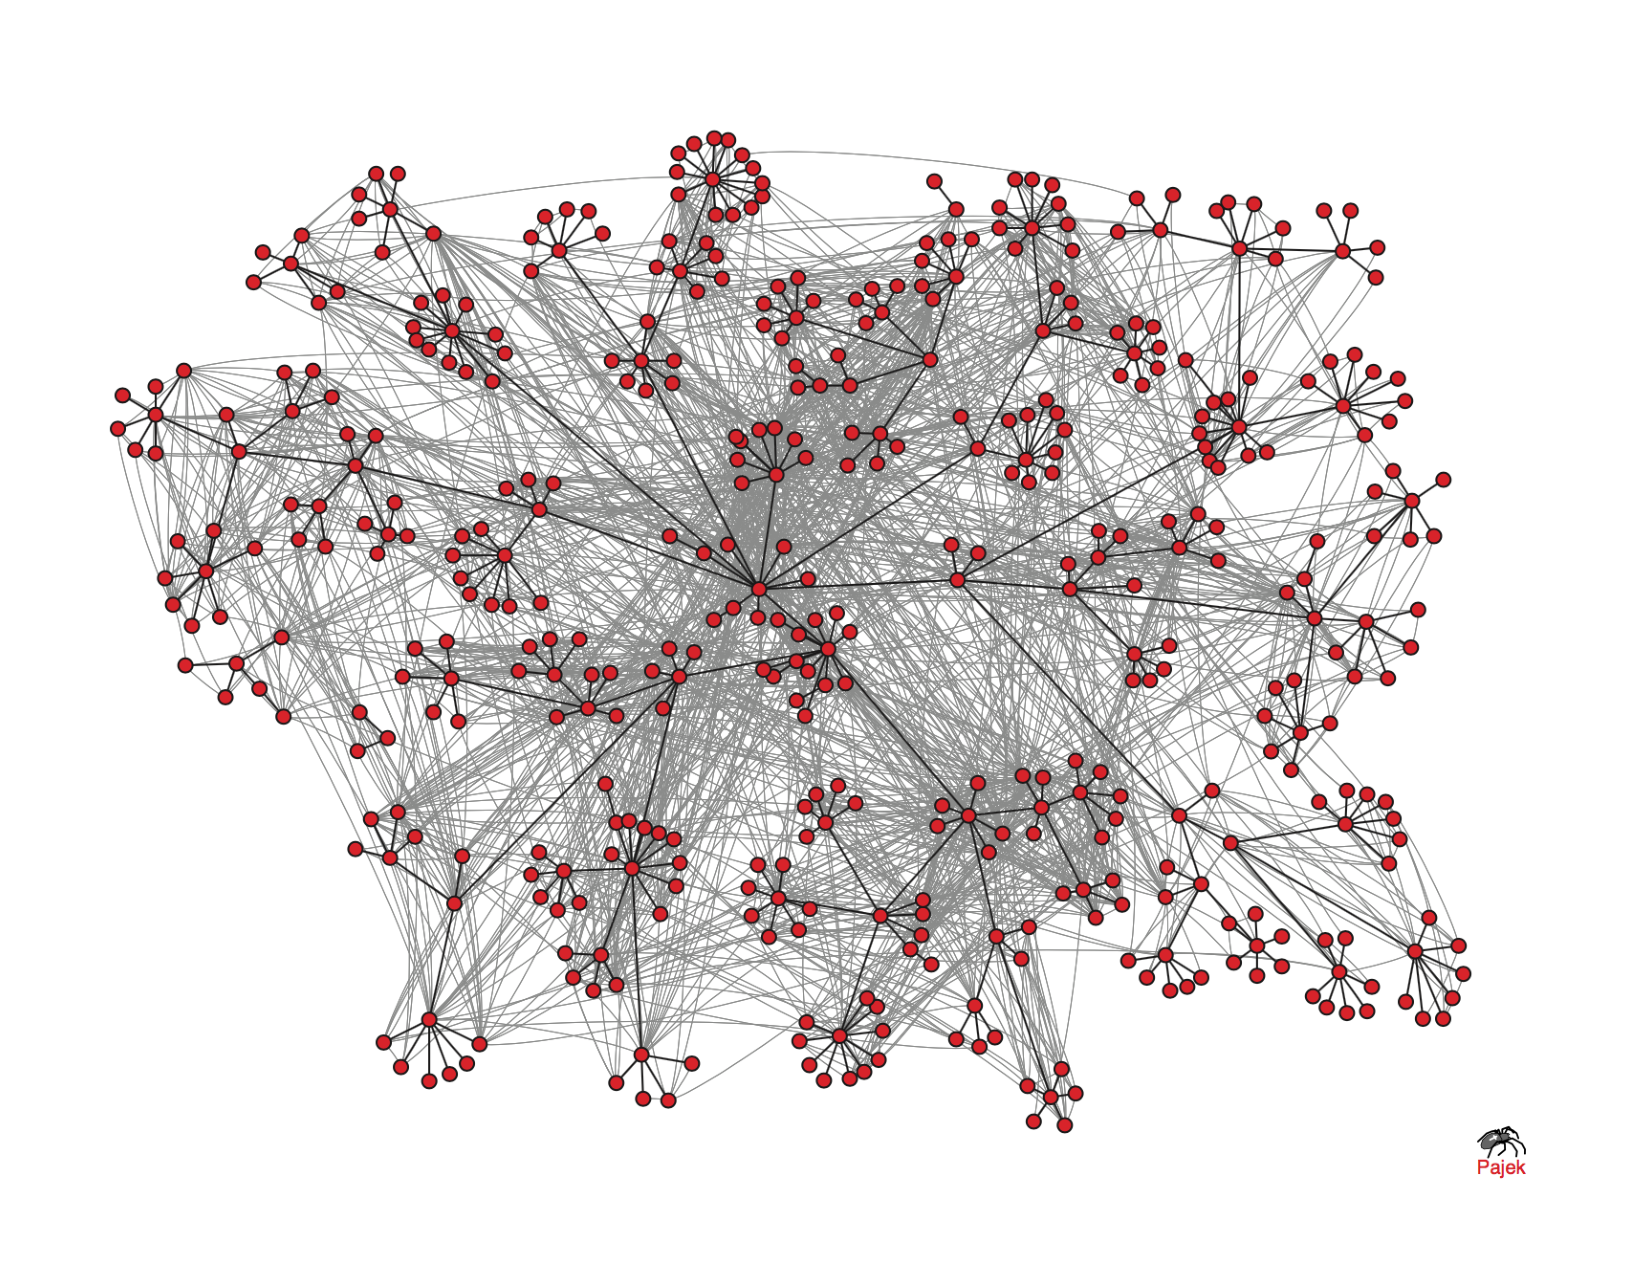
\includegraphics[scale=0.37]{Figs/email}
	\end{figure}
\end{frame}

\begin{frame}{Federal funds network}
	\begin{figure}
	\centering
	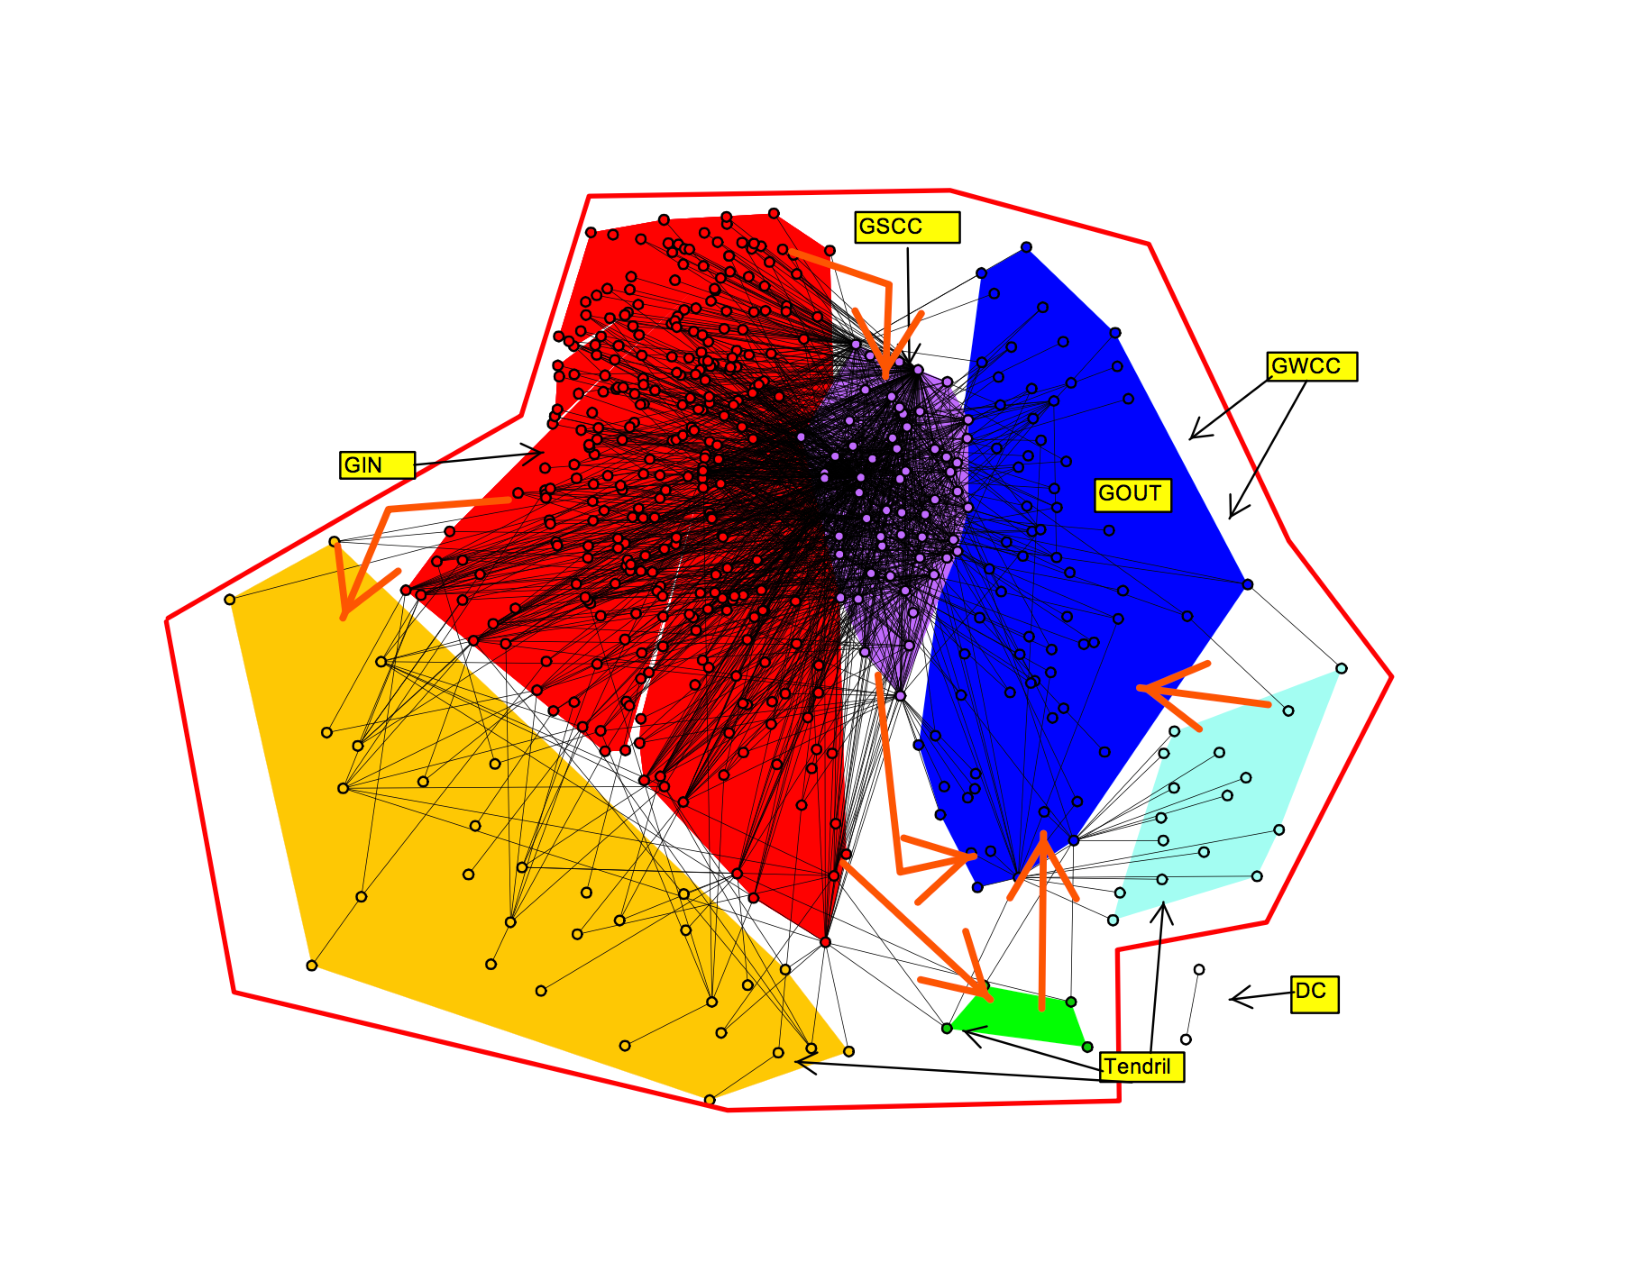
\includegraphics[scale=0.37]{Figs/fed}
	\end{figure}
\end{frame}

\begin{frame}{Inter-marriages between big families in Renaissance Florentine}
	\begin{figure}
	\centering
	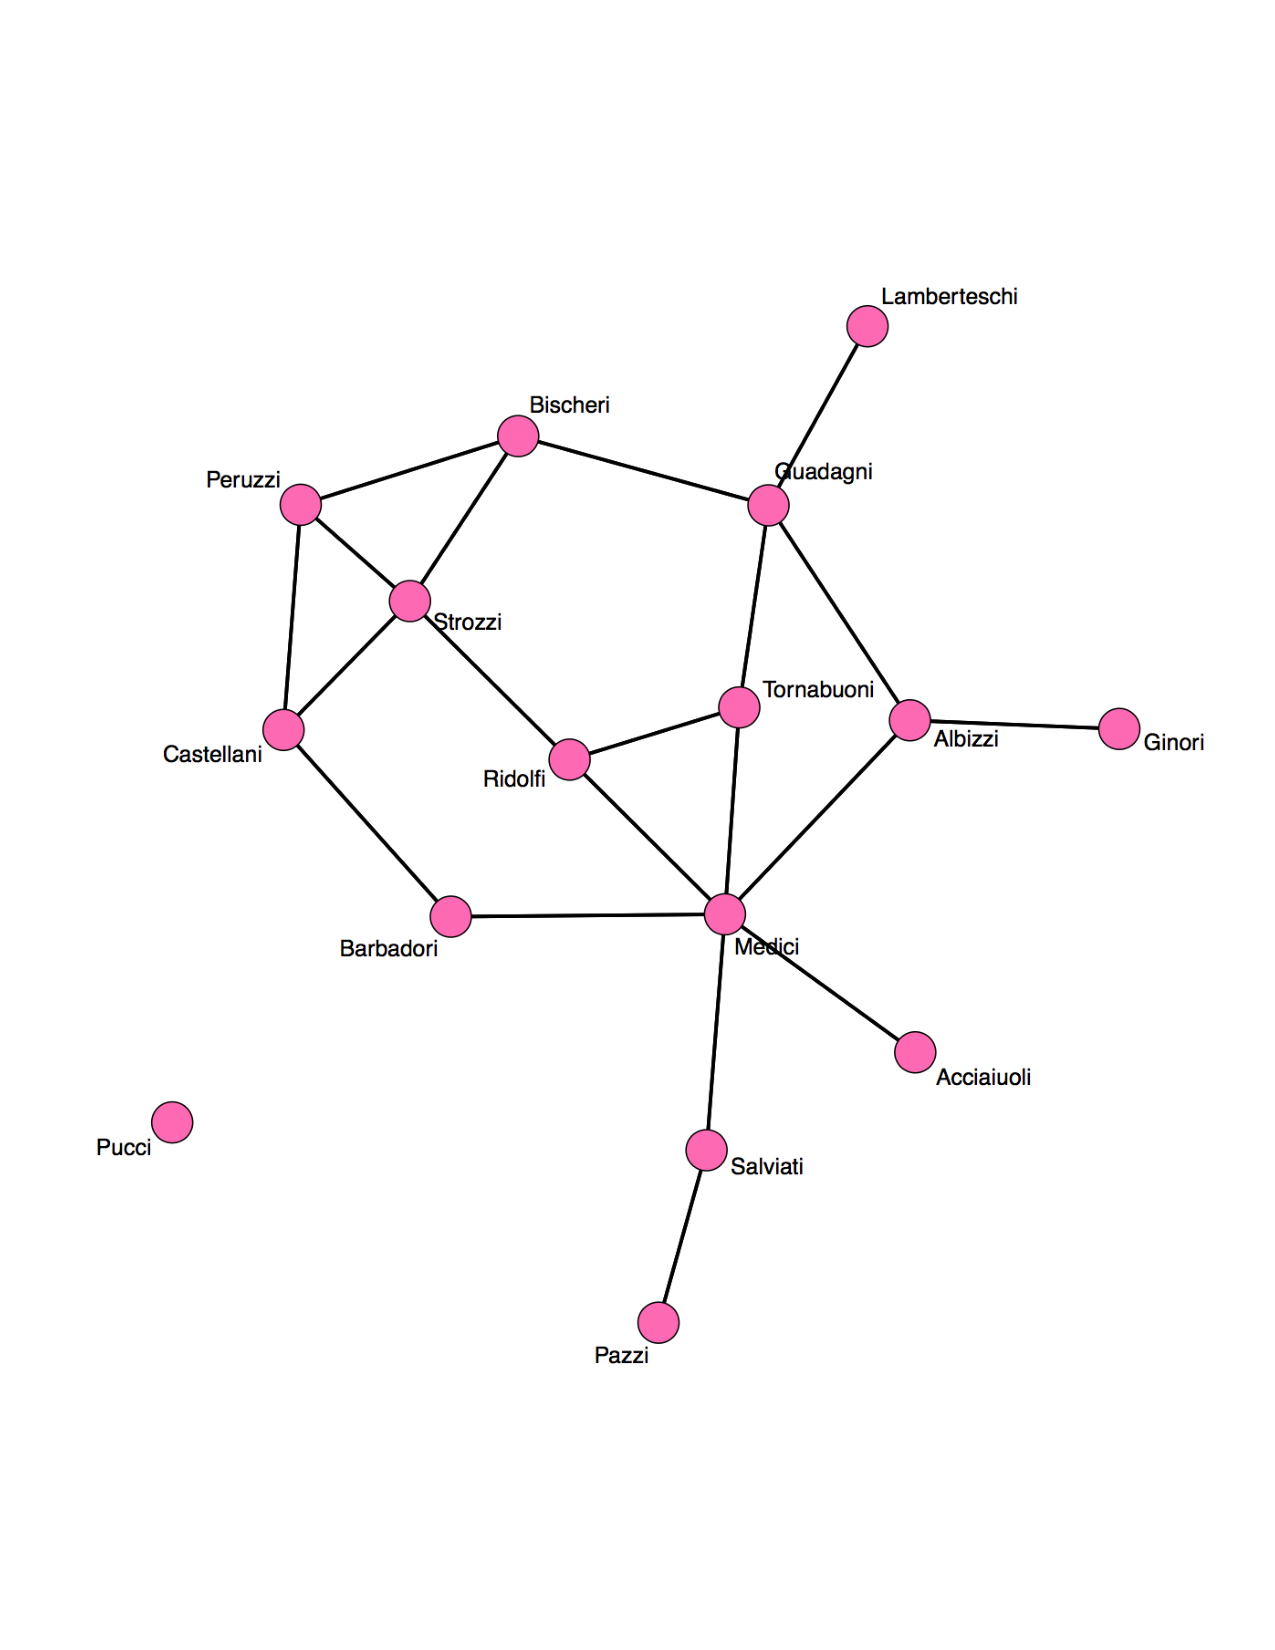
\includegraphics[scale=0.37]{Figs/marriage}
	\end{figure}
\end{frame}

\begin{frame}{Global migration network}
	\begin{figure}
	\centering
	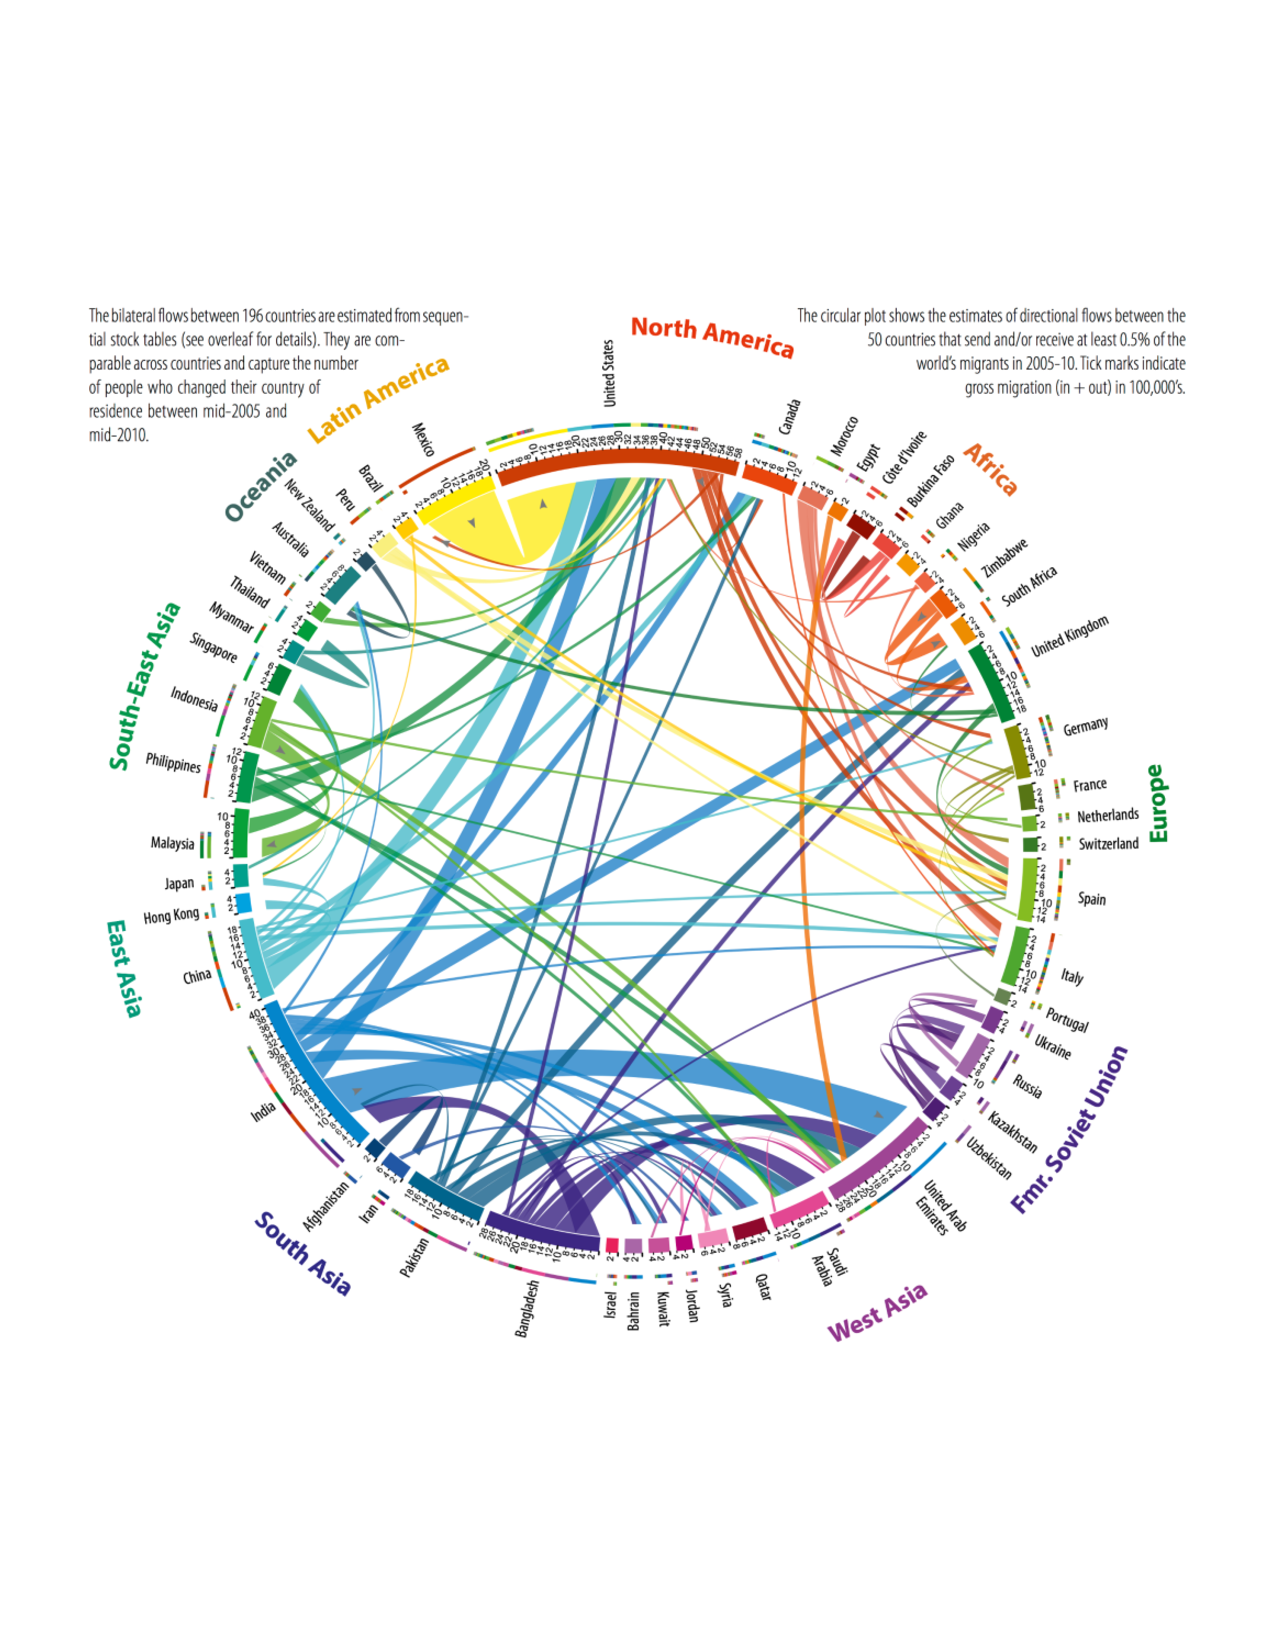
\includegraphics[scale=0.4]{Figs/mig}
	\end{figure}
\end{frame}

\begin{frame}{Network of diseases with shared genes}
	\begin{figure}
	\centering
	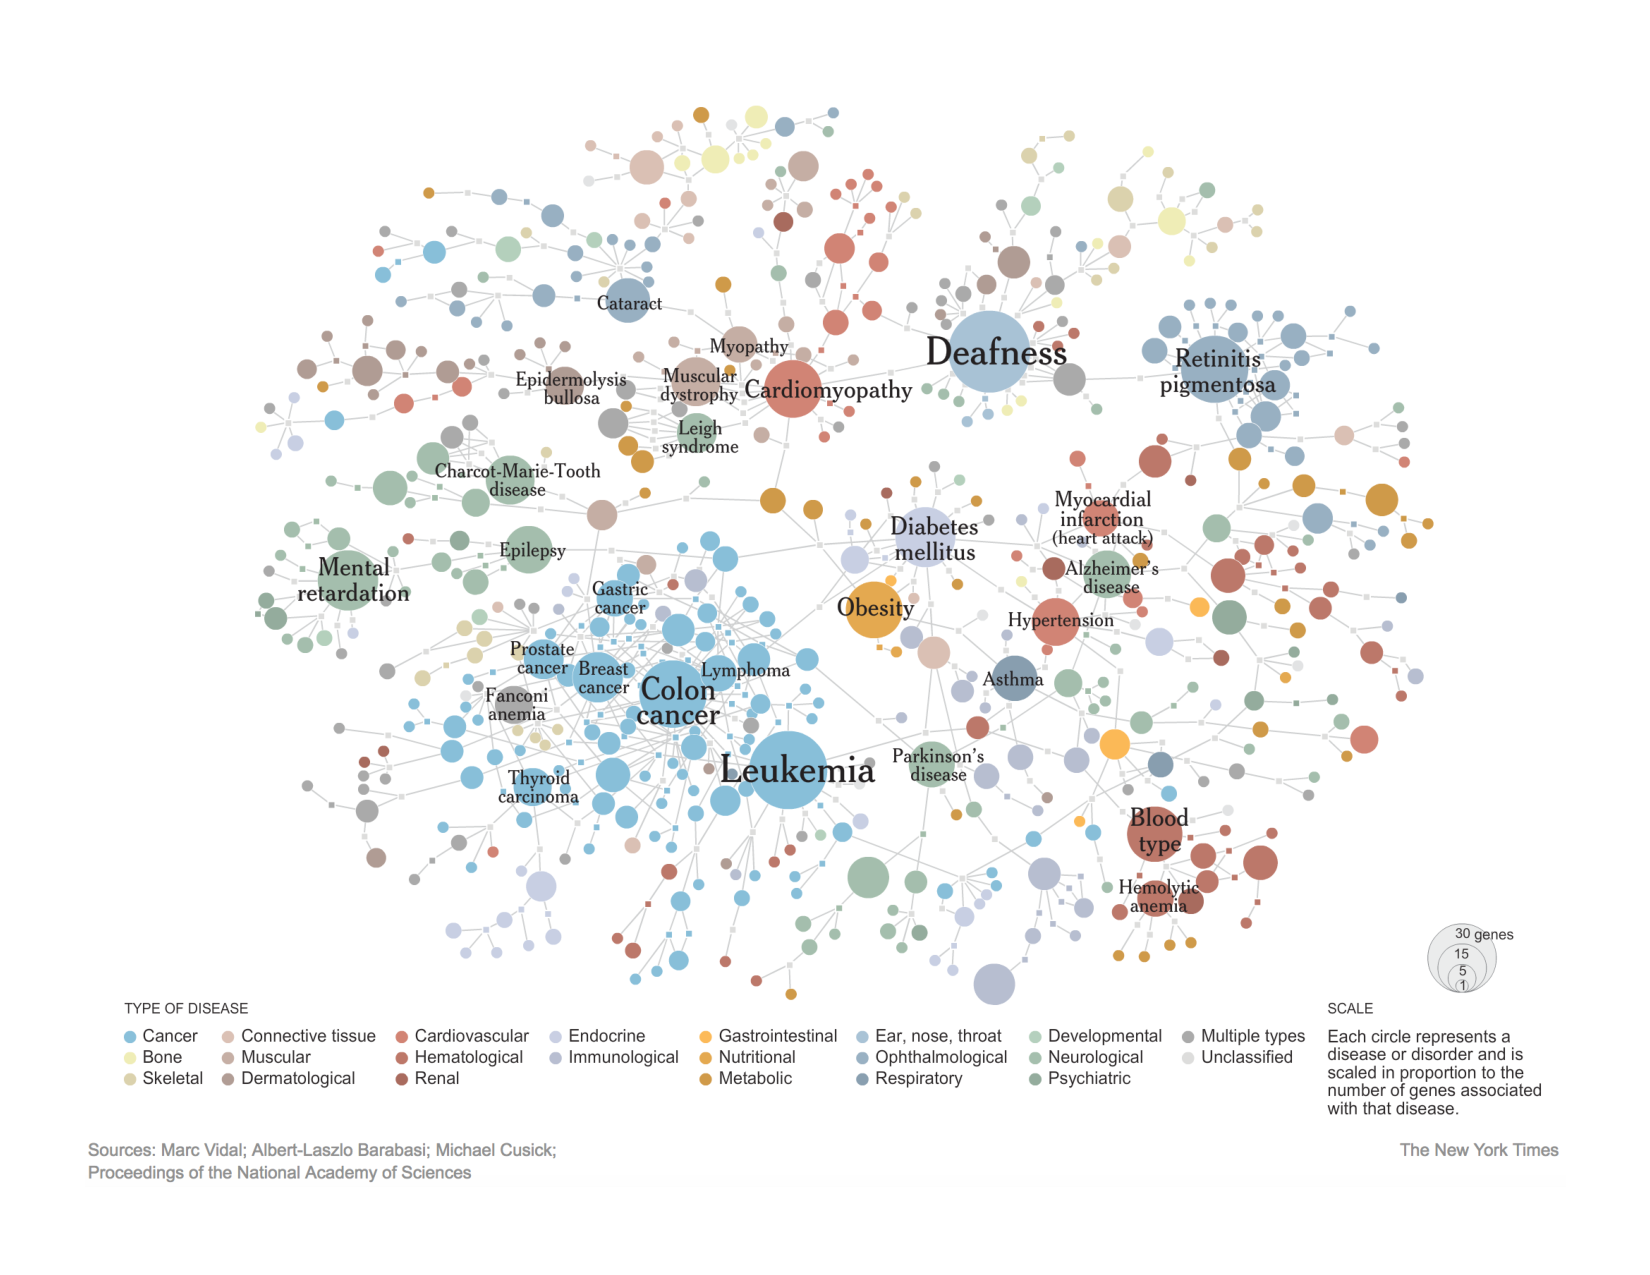
\includegraphics[scale=0.4]{Figs/nyt}
	\end{figure}
\end{frame}

\begin{frame}{Co-mentioned chemicals in articles and patents}
	\begin{figure}
	\centering
	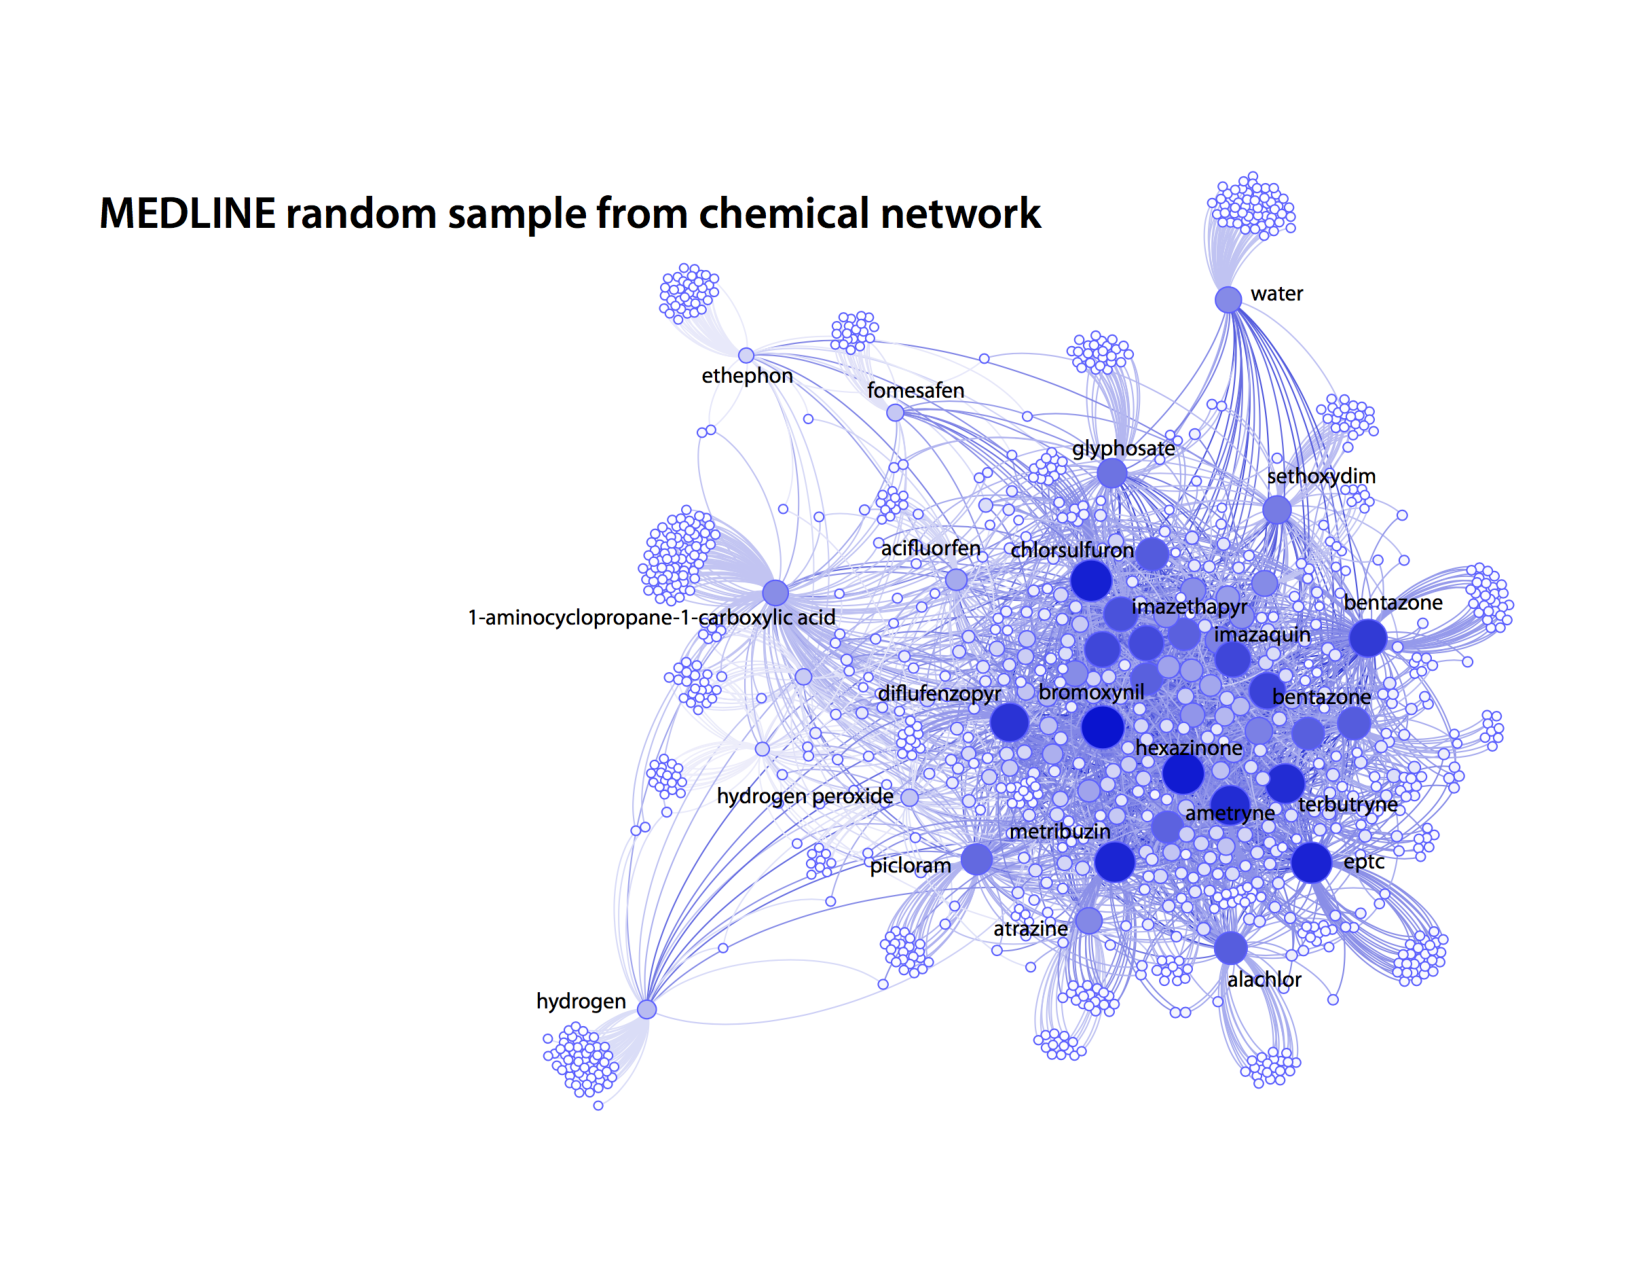
\includegraphics[scale=0.4]{Figs/chem}
	\end{figure}
\end{frame}

\begin{frame}{Network of energy supply in the US}
	\begin{figure}
	\centering
	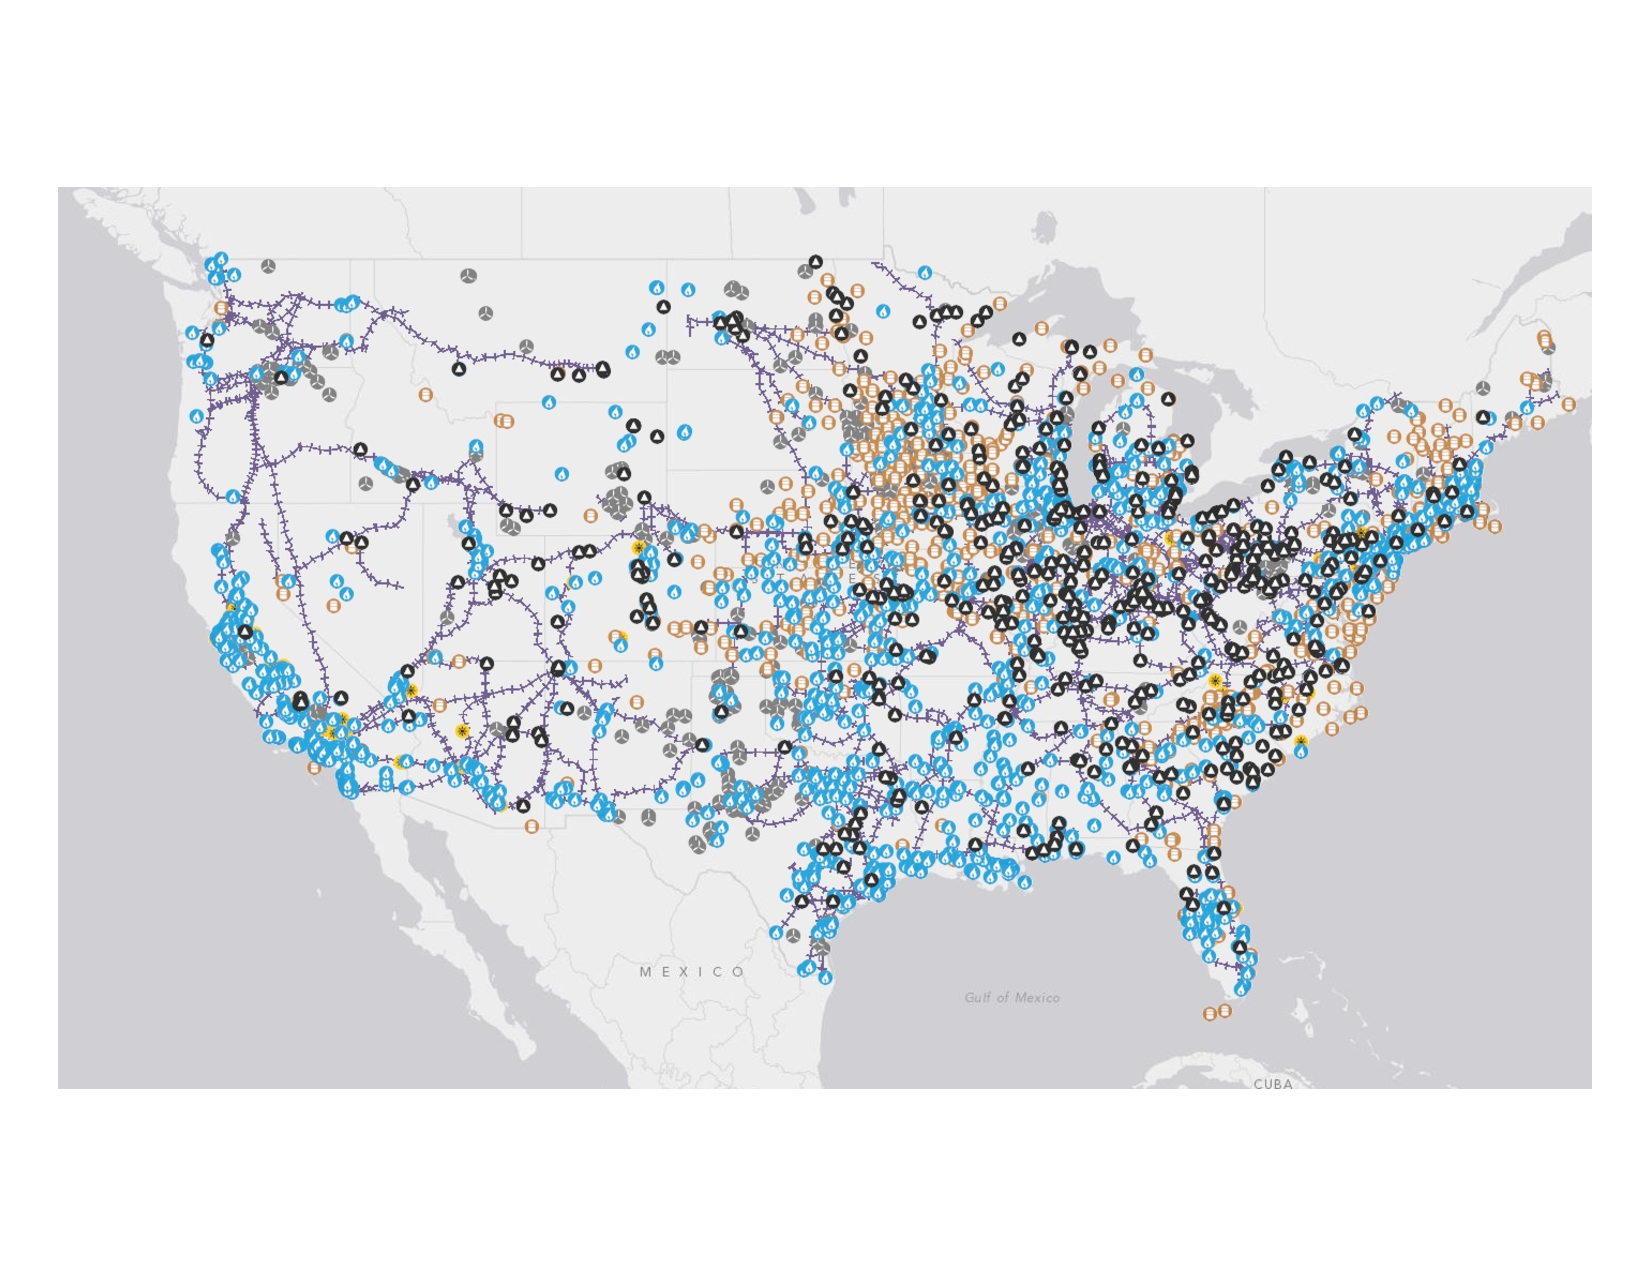
\includegraphics[scale=0.43]{Figs/power}
	\end{figure}
\end{frame}

\begin{frame}{A network and its components}

	\begin{itemize}
		\item Graph (or network)
		\item Nodes (or vertices or actors)
		\item Edges (or links)
	\end{itemize}
\end{frame}

\begin{frame}
	\begin{figure}
	\centering
	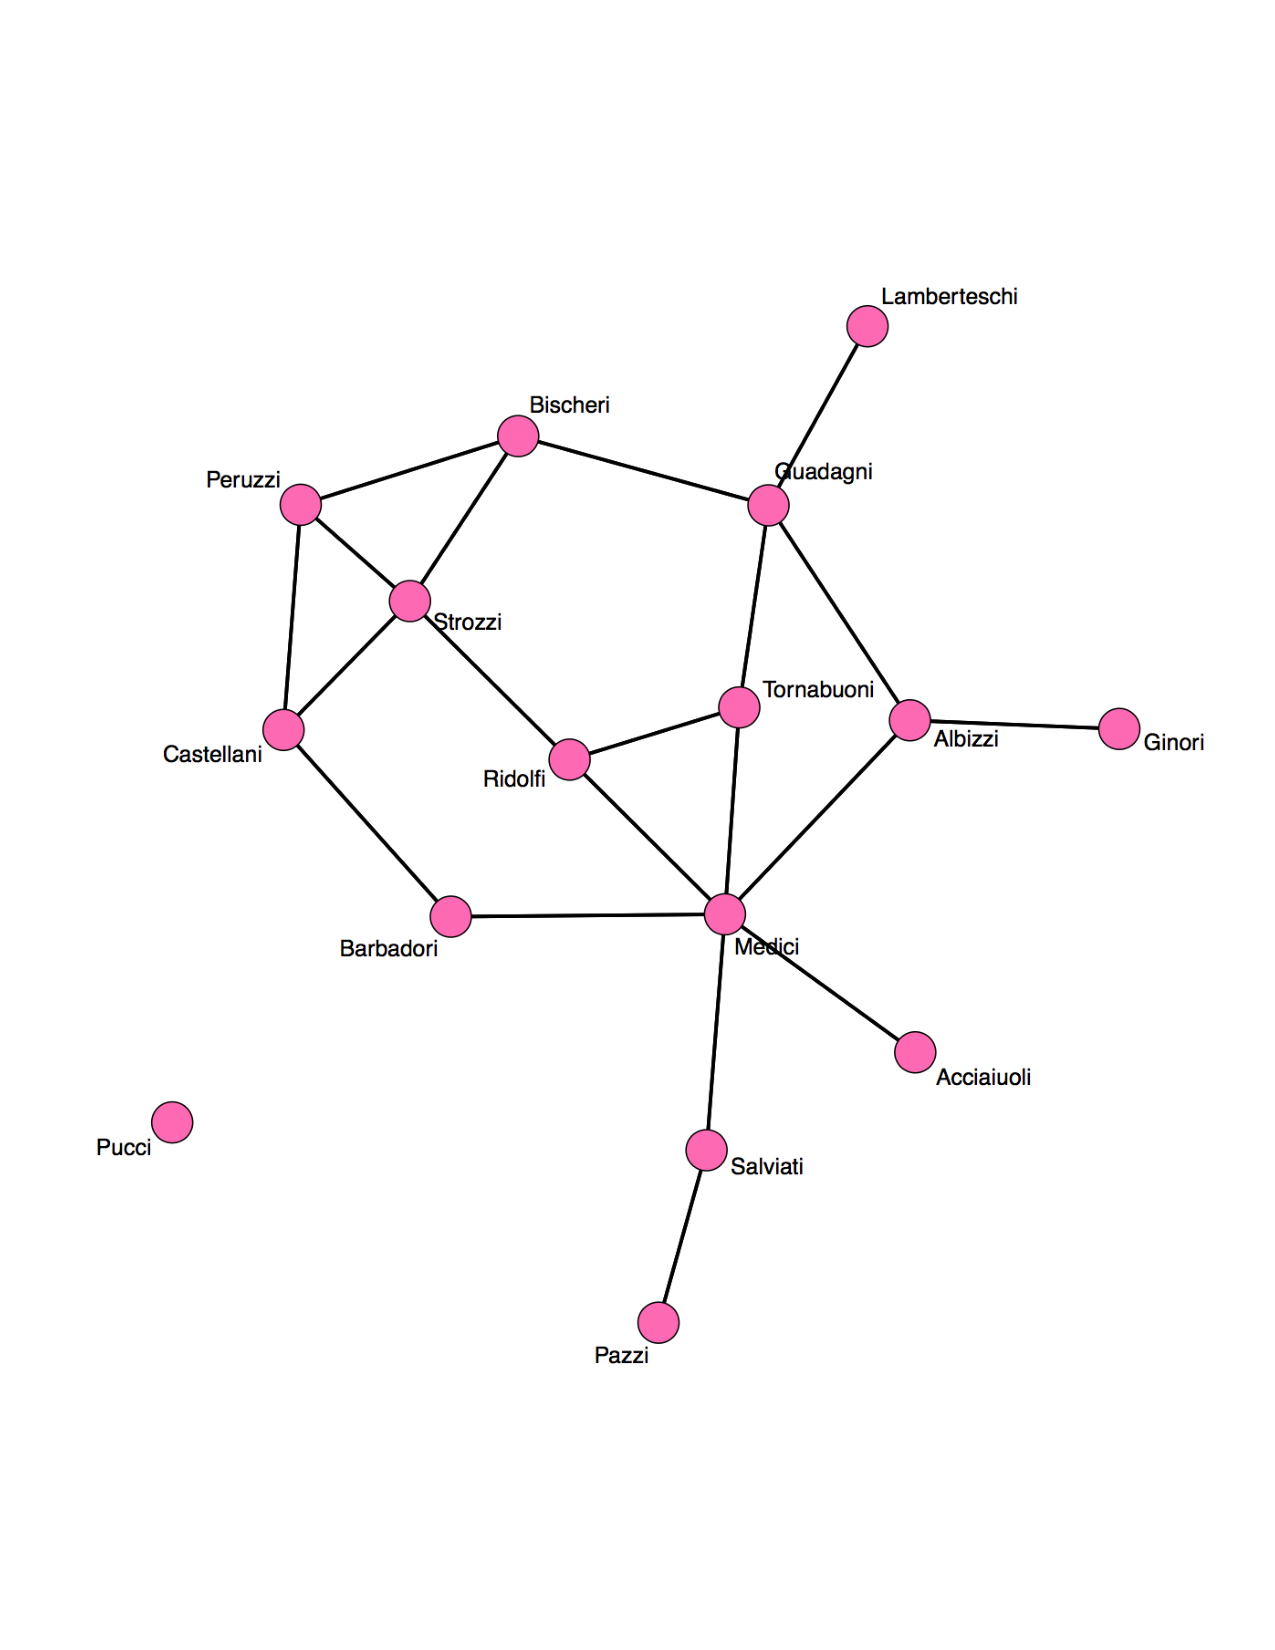
\includegraphics[scale=0.37]{Figs/marriage}
	\end{figure}
\end{frame}

\begin{frame}{A network and its components}
	\begin{itemize}
		\item A \textbf{graph} (\textbf{network}) is a composed of a set of objects, called \textbf{nodes} or \textbf{vertices}, with certain pairs of these objects connected by \textbf{links} called \textbf{edges}.
		
		\item Two nodes are \textbf{neighbors} if they are connected by an edge.
	\end{itemize}
\end{frame}

\begin{frame}{Adjacency matrix: Math representation of networks}
The adjacency matrix or sociomatrix \textbf{A} of a \textit{simple} graph (network) is an $n\times n$ matrix with elements
	\begin{equation}
	A_{ij} =
	\begin{cases}
	1 & \text{if there exists an edge between $i$ and $j$}\\
	0 & \text{otherwise},
	\end{cases}
	\end{equation}
where $n$ refers to the number of \textbf{nodes}.
\end{frame}

\begin{frame}
	\begin{figure}
	\centering
	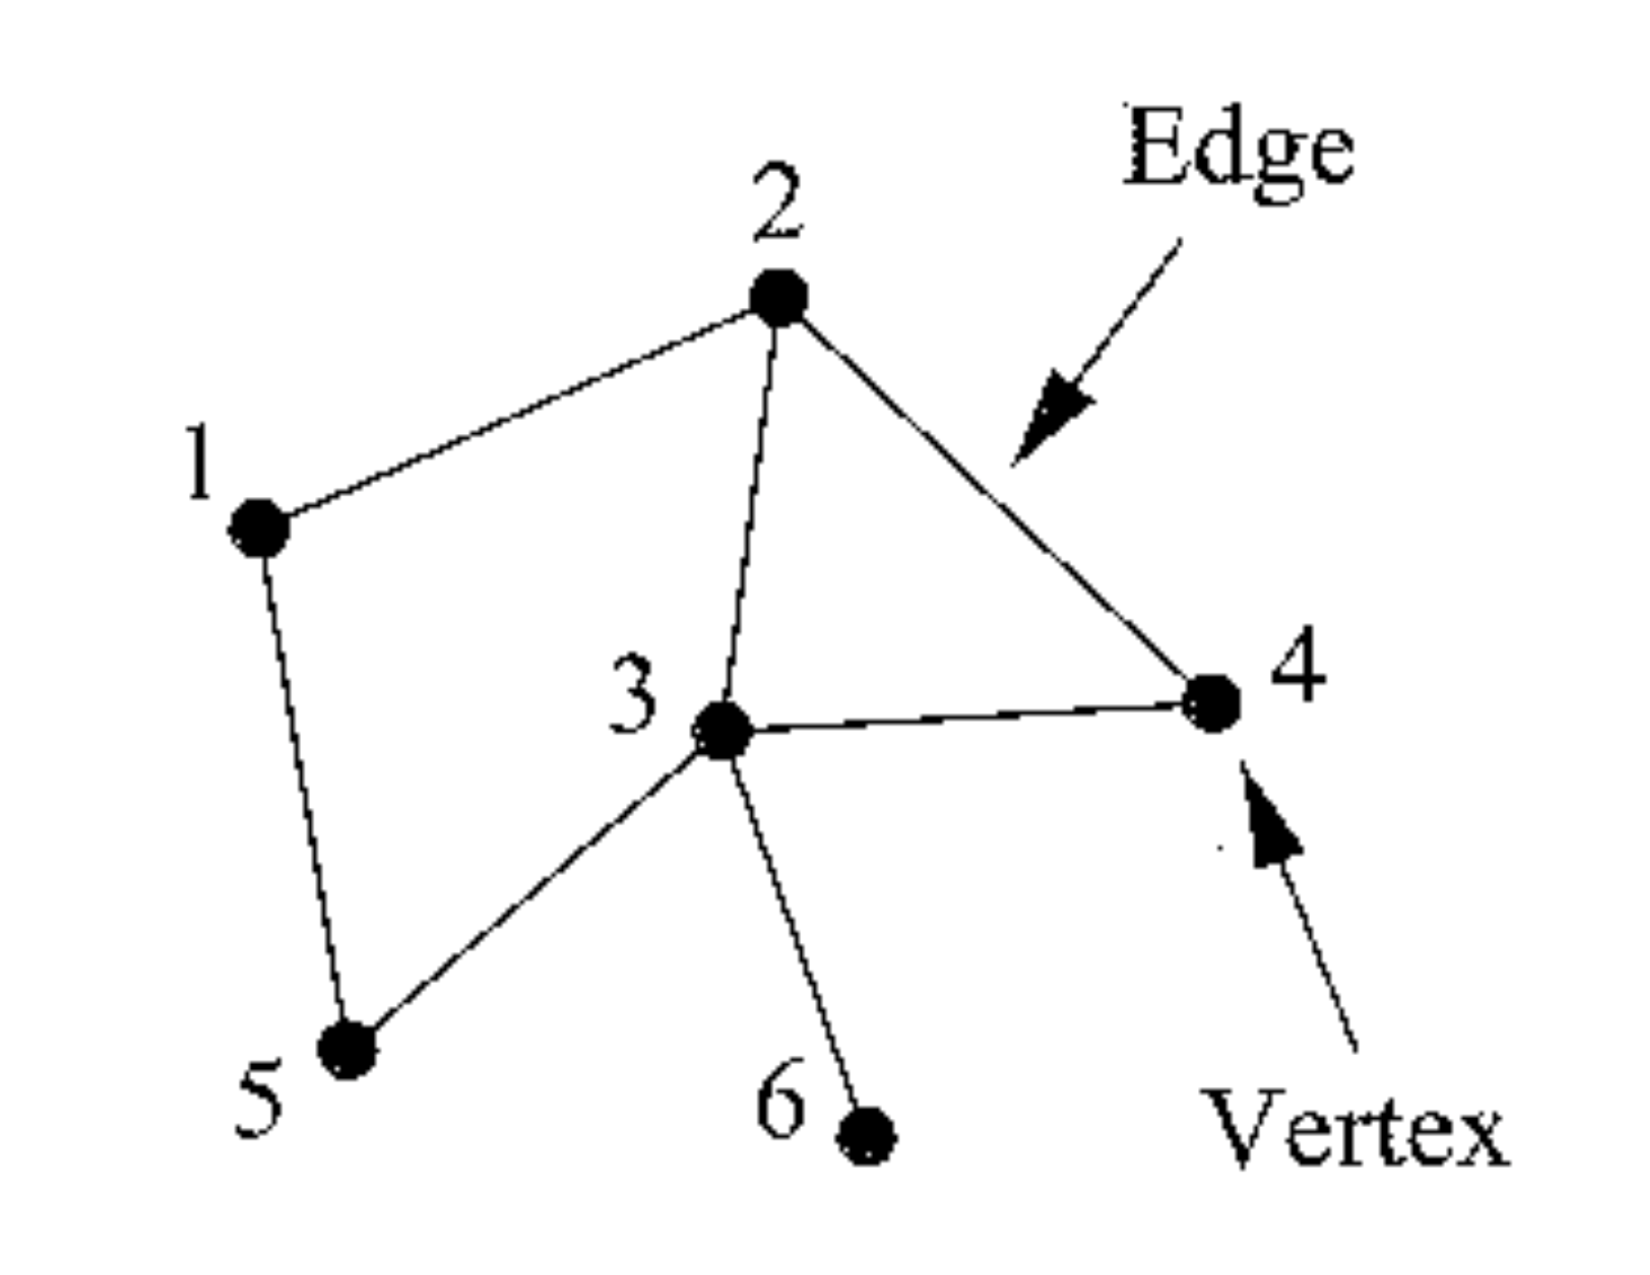
\includegraphics[scale=0.2]{Figs/ex}
	\end{figure}
	\vspace{0.2cm}
	\begin{equation}
	A =
	\begin{bmatrix}
	0 & 1 & 0 & 0 & 1 \\
	1 & 0 & 1 & 1 & 0 \\
	0 & 1 & 0 & 1 & 1 \\
	0 & 1 & 1 & 0 & 0 \\
	1 & 0 & 1 & 0 & 0		
	\end{bmatrix}
	\end{equation}

\vspace{0.2cm}
What is unique about this matrix?
\end{frame}

\begin{frame}{Types of networks I: Simple graph}
A network that has neither self-edges nor multiedges. Formally speaking, in addition to the definition above,

	\begin{equation}
	A_{ii} = 0 \quad \forall \quad i.
	\end{equation}
\end{frame}

\begin{frame}
	\begin{figure}
	\centering
	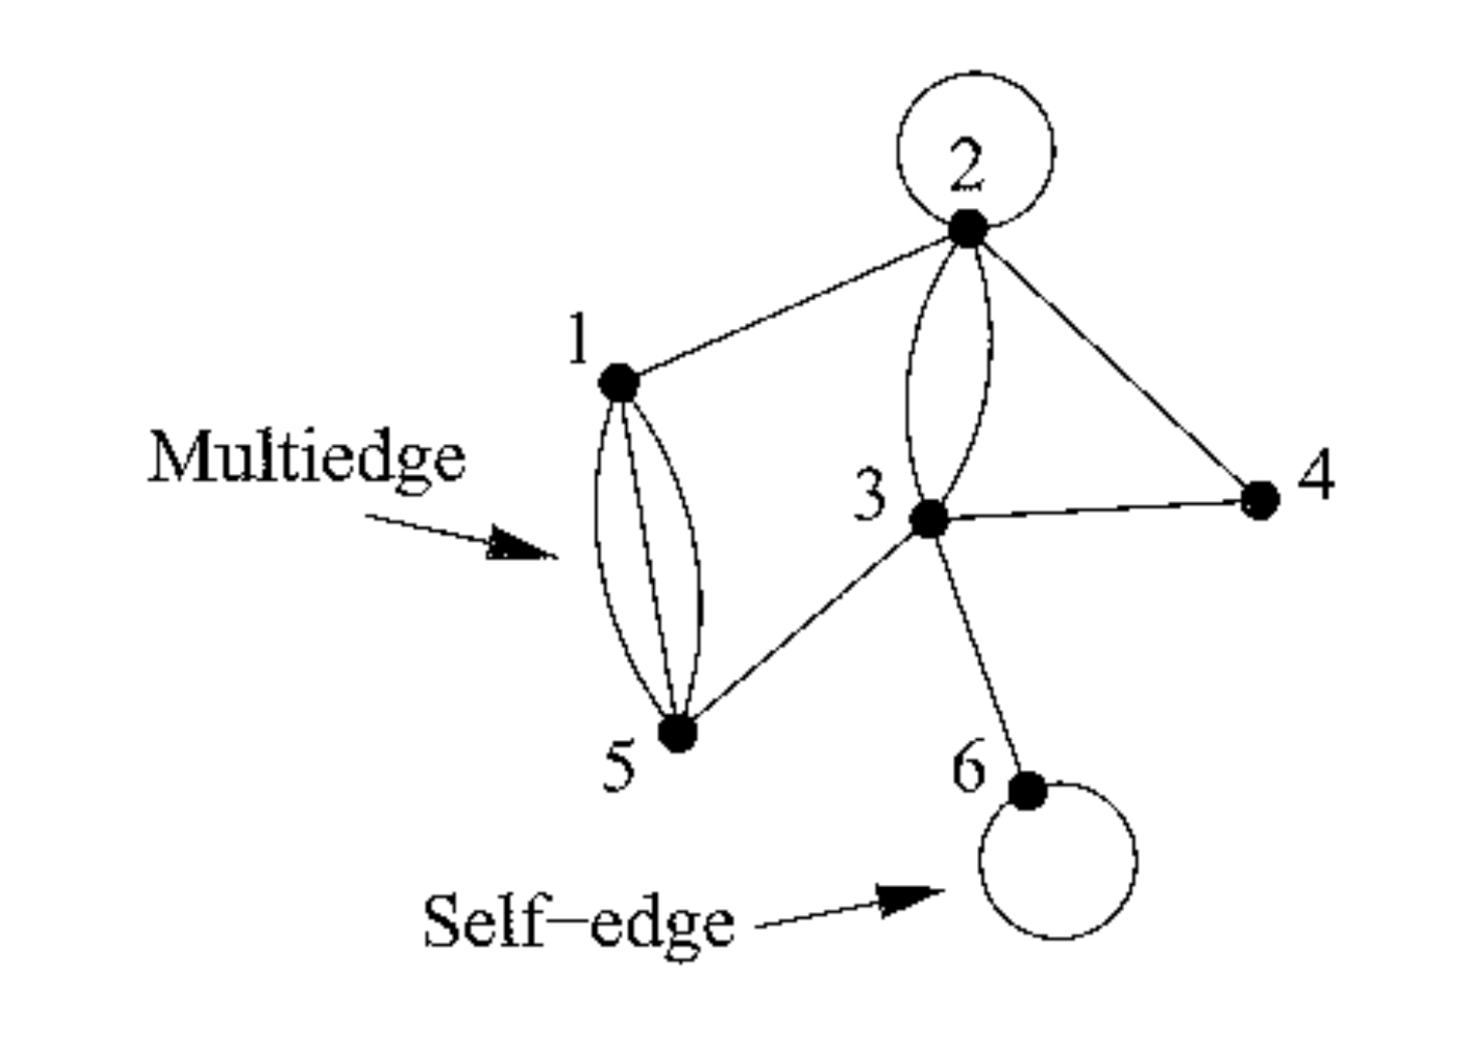
\includegraphics[scale=0.35]{Figs/weird}
	\end{figure}
\end{frame}

\begin{frame}{Types of networks II: Weighted network}
The adjacency matrix or sociomatrix \textbf{A} of a weighted network is an $n\times n$ matrix with elements
	\begin{equation}
	A_{ij} =
	\begin{cases}
	r \in \mathbb{R} & \text{if there exists an edge between $i$ and $j$}\\
	0 & \text{otherwise},
	\end{cases}
	\end{equation}
where $n$ refers to the number of \textbf{nodes}.\\

\vspace{1cm}
Examples?
\end{frame}

\begin{frame}{Types of networks III: Directed graph}
A directed network is a network in which edges have a direction, pointing from one vertex to another. The adjacency matrix \textbf{A} of a \textit{directed} graph is the matrix with elements
	\begin{equation}
	A_{ij} =
	\begin{cases}
	1 & \text{if there exists an edge from $j$ and $i$}\\
	0 & \text{otherwise},
	\end{cases}
	\end{equation}
where $n$ refers to the number of \textbf{nodes}.\\

\vspace{1cm}
Examples?
\end{frame}

\begin{frame}
	\begin{figure}
	\centering
	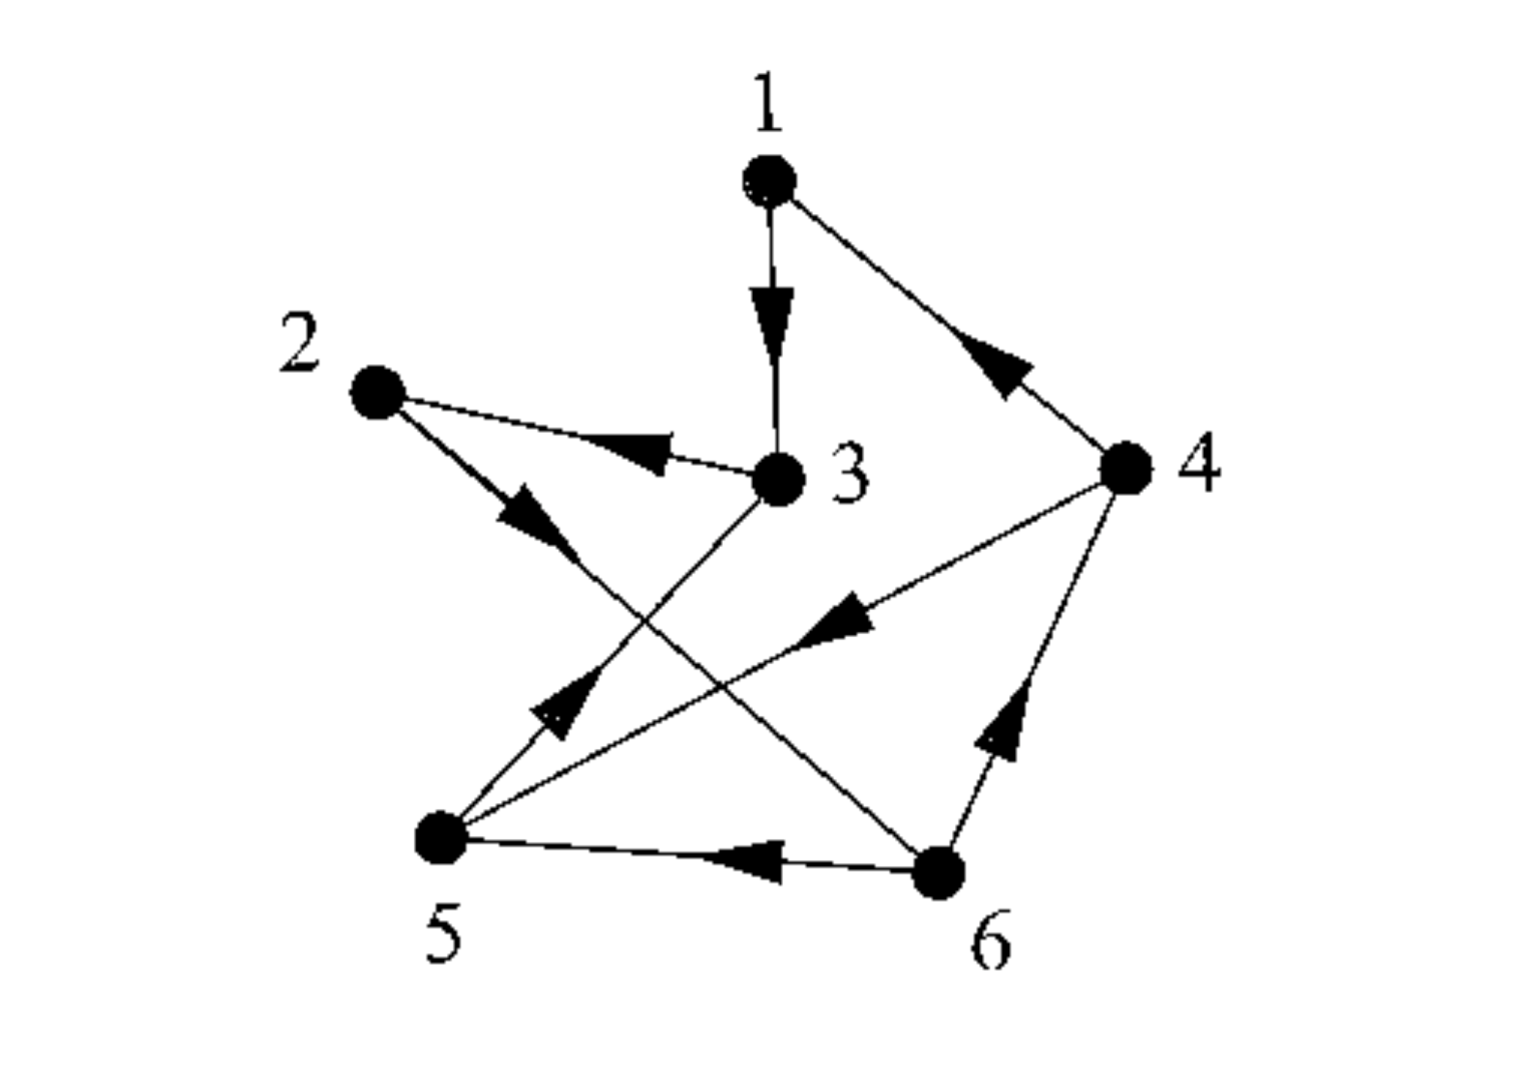
\includegraphics[scale=0.2]{Figs/dig}
	\end{figure}
	\vspace{0.2cm}
	\begin{equation}
	A =
	\begin{bmatrix}
	0 & 0 & 0 & 1 & 0 & 0 \\
	0 & 0 & 1 & 0 & 0 & 0 \\
	1 & 0 & 0 & 0 & 1 & 0 \\
	0 & 0 & 0 & 0 & 0 & 1 \\
	0 & 0 & 0 & 1 & 0 & 1 \\
	0 & 1 & 0 & 0 & 0 & 0		
	\end{bmatrix},
	\end{equation}
 in which columns and rows refer to the starting and ending points respectively. 
\end{frame}

\begin{frame}
	\begin{figure}
	\centering
	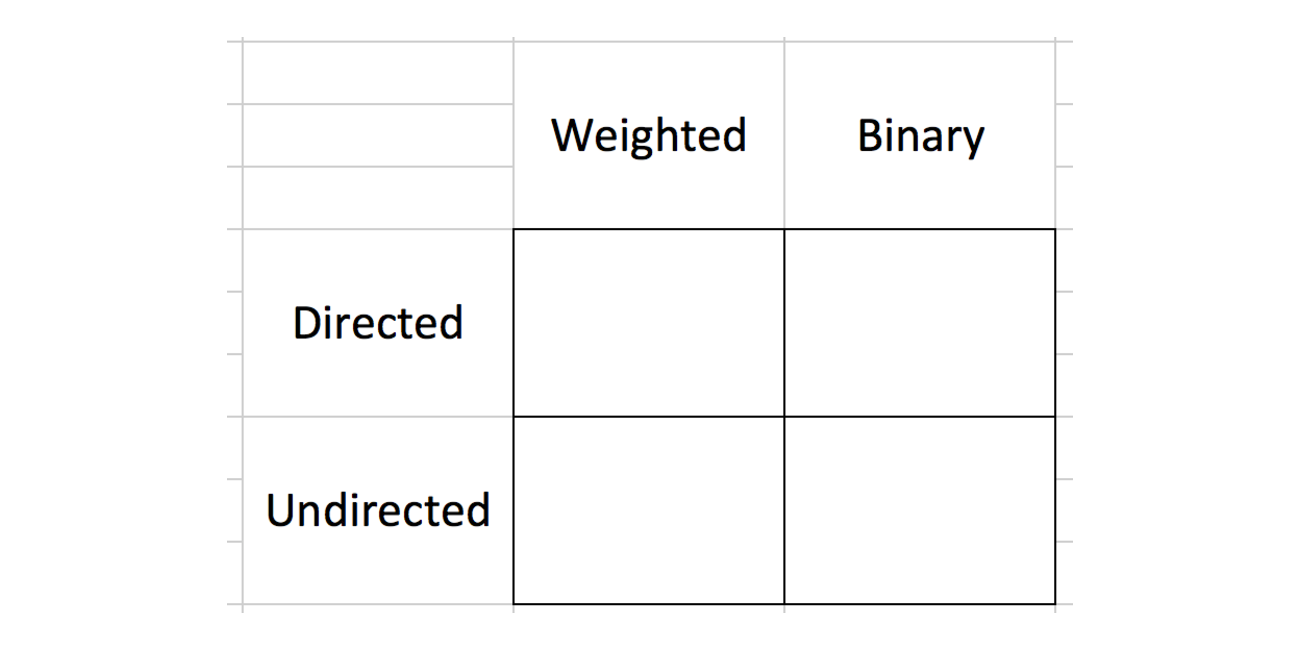
\includegraphics[scale=0.43]{Figs/typeb}
	\end{figure}
\end{frame}

\begin{frame}
	\begin{figure}
	\centering
	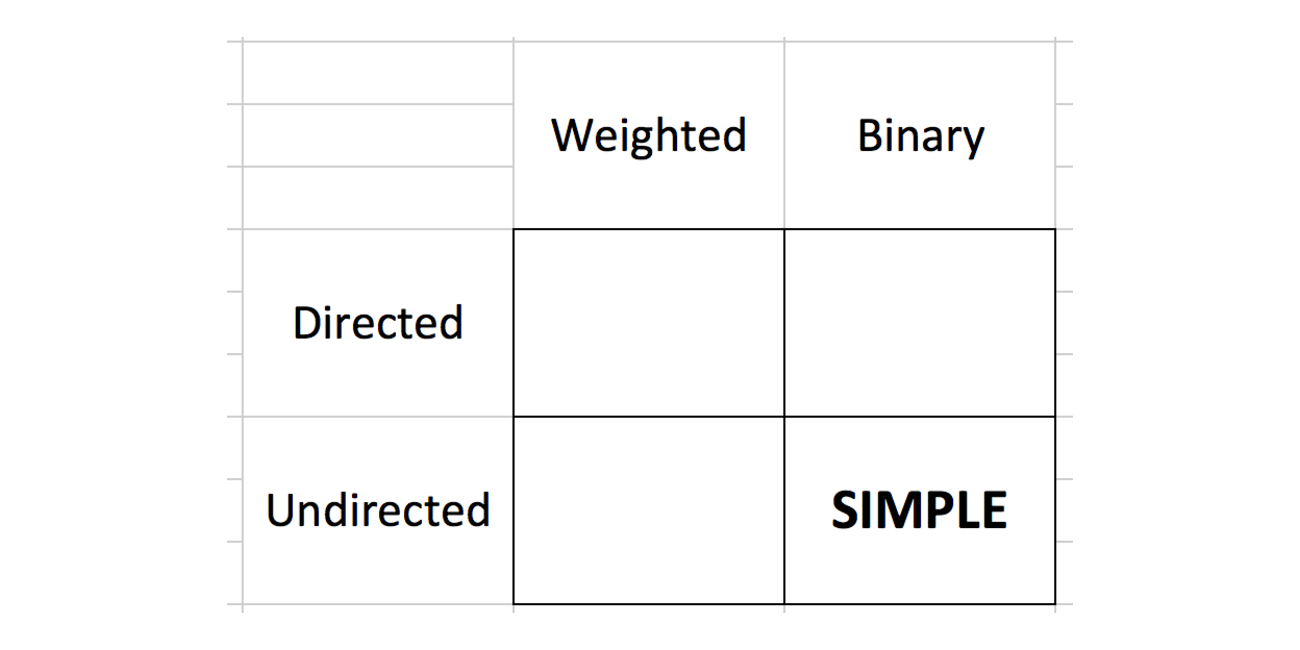
\includegraphics[scale=0.43]{Figs/typea}
	\end{figure}
\end{frame}

\begin{frame}{Types of networks IV: Affiliation network}
	\begin{itemize}
		\item A \textbf{bipartite graph} is a graph in which there are two types of node, and edges only run between the two types.
		
		\item A \textbf{hypergraph} is a network in which edges can join two or more nodes.
	\end{itemize}
\end{frame}

\begin{frame}
	\begin{figure}
	\centering
	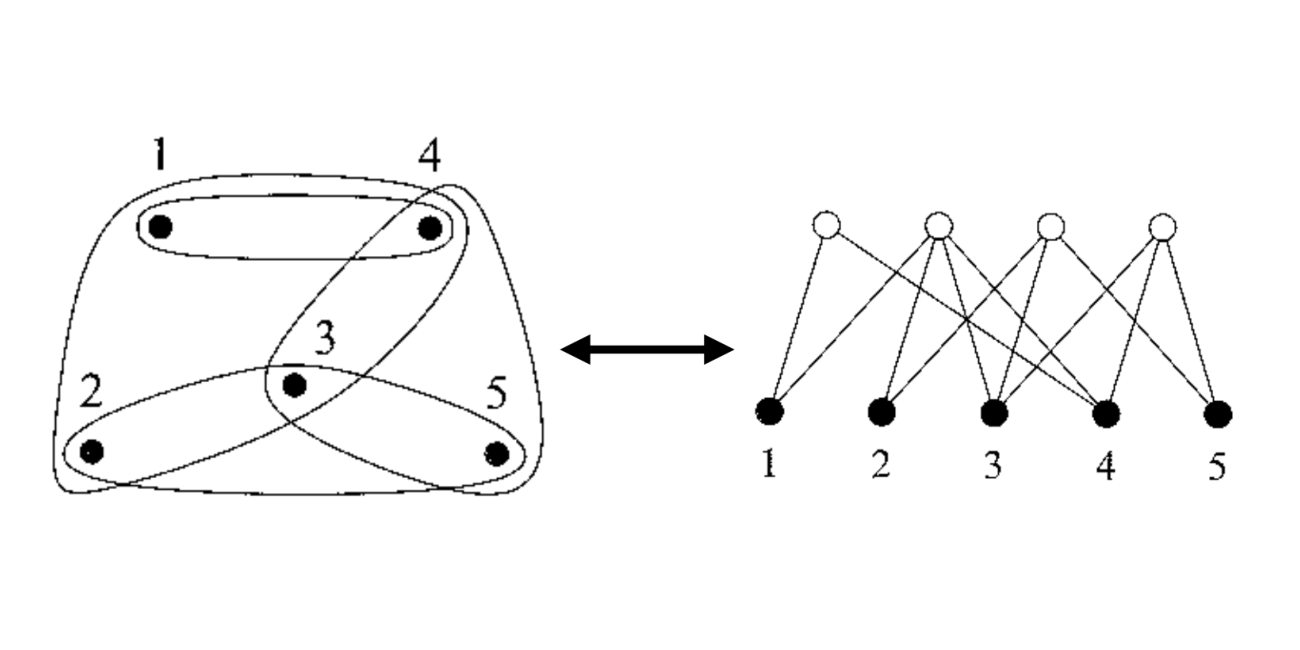
\includegraphics[scale=0.5]{Figs/bihy}
	\end{figure}
	\vspace{0.2cm}
	\begin{equation}
	B =
	\begin{bmatrix}
	1 & 0 & 0 & 1 & 0 \\
	1 & 1 & 1 & 1 & 0 \\
	0 & 1 & 1 & 0 & 1 \\
	0 & 0 & 1 & 1 & 1 \\
	\end{bmatrix},
	\end{equation}
where rows correspond to groups and columns refer to actors.
\end{frame}

\begin{frame}{Types of networks IV: Affiliation network}
One-mode projection: From bipartite graph to simple graph.
	\begin{equation}
	P_{ij} = \sum_{k=1}^g B_{ki}B_{kj} = \sum_{k=1}^g B_{ik}^{T}B_{kj},
	\end{equation}
where $k$ refers to affiliated groups.
\end{frame}

\begin{frame}{Types of networks: Others}
	\begin{itemize}
		\item Cocitation network (i.e., studies that are cited together in other studies).
		\item Bibliographic coupling network (i.e., studies that use the same references).
		\item Regular network (i.e., networks in which all nodes have the same degree).
		\item Planar network (i.e., networks that can be visualized without any edges crossing each other).		
		\item Tree and forest.
		\item ... and more.
	\end{itemize}
\end{frame}

\begin{frame}{Social network analysis (SNA): Two pillars}
	\begin{itemize}
		\item Descriptive: Study numerical summary measures of networks
		\item Generative: Study underlying dynamic process of network formation; hypothesis testing; simulation (e.g., ERGM)
	\end{itemize}
\end{frame}

\begin{frame}{Descriptive SNA}
	\begin{itemize}
		\item Network connectivity
			\begin{itemize}
			\item Degree
			\item Density
			\item Path and geodesic distance
			\end{itemize}
		\item Node centrality: Measures of node importance in a network
		\item ... and more (e.g., cosine similarity, cliques, triads, assortive mixing)
	\end{itemize}
\end{frame}

\begin{frame}{Descriptive SNA I: Degree}
Given an adjacency matrix \textbf{A}, the degree of a vertex is the number of edges connected to it.
	\begin{equation}
	k_i  = \sum_j^n A_{ij},
	\end{equation}
where $n$ refers to the number of nodes in the graph.
\end{frame}

\begin{frame}{Descriptive SNA I: Degree}
The total number of edges in graph \textbf{A} will be
	
	\begin{equation}
	\begin{split}
	& 2m = \sum_i^n k_i\\
	\Rightarrow \quad & m = \frac{1}{2} \sum_i^n k_i
	\end{split}
	\end{equation}
\end{frame}

\begin{frame}{Descriptive SNA I: Degree}
How do we derive the mean degree of graph \textbf{A}?
	
	\begin{equation}
	c = \frac{1}{n} \sum_i^n k_i = \frac{2m}{n}
	\end{equation}
\end{frame}

\begin{frame}{Descriptive SNA I: Degree}
	\begin{itemize}
		\item A \textbf{regular} graph is one in which all nodes have the same degree.
	\end{itemize}
\end{frame}

\begin{frame}
	\begin{figure}
	\centering
	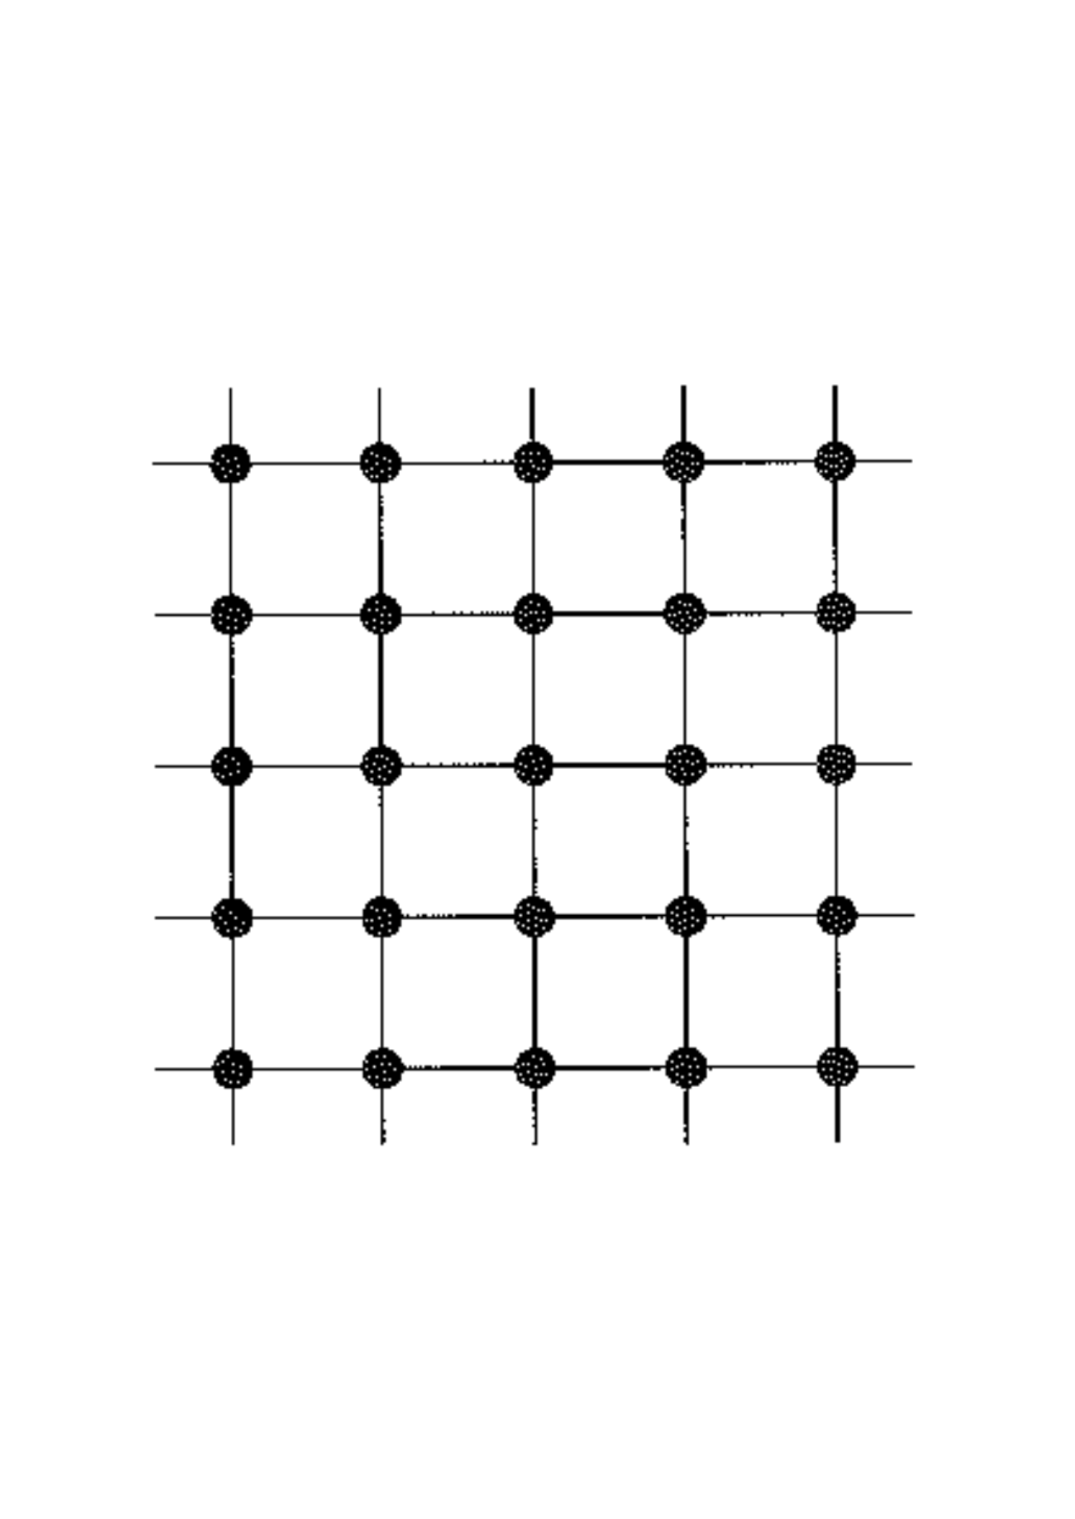
\includegraphics[scale=0.5]{Figs/reg}
	\end{figure}
\end{frame}

\begin{frame}{Descriptive SNA II: Density}
	\begin{itemize}
		\item The density of a graph measures the \textit{connectance} of a graph.
		
		\item Mathematically, it is defined as the number of edges out of the max possible number of edges of a graph.
	\end{itemize}
\end{frame}

\begin{frame}{Descriptive SNA II: Density}
Mathematically, it is defined as the share of the number of edges out of the max possible number of edges of a graph.

	\begin{equation}
	\rho = \frac{m}{\binom{n}{2}}  = \frac{m}{\frac{1}{2} n(n-1)} = \frac{2m}{n(n-1)}  = \frac{c}{n-1},
	\end{equation}
where $c$ is the mean degree.\\

\vspace{0.3cm}
What is the big deal here?	
\end{frame}

\begin{frame}{Descriptive SNA II: Density}
	\begin{itemize}
		\item A network for which the density tends to a constant as the number of nodes tends to infinity is \textbf{dense}. That is, $\rho$ remains constant as $n \to \infty$.
		
		\item A network for which the density tends to 0 as the number of nodes tends to infinity is \textbf{sparse}. That is, $\rho \to 0$ as $n \to \infty$.
	\end{itemize}
\end{frame}

\begin{frame}{Descriptive SNA III: Path, walk, and distance}
	\begin{itemize}
		\item A \textbf{path} is a sequence of nodes with the property that each consecutive pair in the sequence is connected by an edge.
		\item A \textbf{simple path} is a sequence of nodes with the property that each consecutive pair in the sequence is connected by an edge and each node in the sequence appears only once.
	\end{itemize}
\end{frame}

\begin{frame}{Descriptive SNA III: Path, walk, and distance}
	\begin{itemize}
		\item In statistics, a path is also a \textbf{walk}.
		
		\item A \textbf{walk} of length $k$ between nodes $i$ and $j$ means that the path between $i$ and $j$ contains $k$ edges where $i\neq j$.
	\end{itemize}
\end{frame}

\begin{frame}{Descriptive SNA III: Path, walk, and distance}
\begin{itemize}
	\item Existence of \textit{walks} between nodes tell us about network connectivity.
	
	\item Existence of \textit{walks of minimal length} tells us about \textbf{geodesics}, or geodesic distance, between two nodes in the graph.
\end{itemize}

Walks of all lengths between a pair of nodes can be counted using matrix multiplication.
\end{frame}

\begin{frame}{Descriptive SNA III: Path, walk, and distance}
Define $W = A^k$, where $k$ means we multiply the adjacency matrix of graph \textbf{A} for $k$ times, then 
	\begin{equation}
	W_{ij} = \text{the number of walks of length $k$ between $i$ and $j$.}	
	\end{equation}
\end{frame}

\begin{frame}
	\begin{figure}
	\centering
	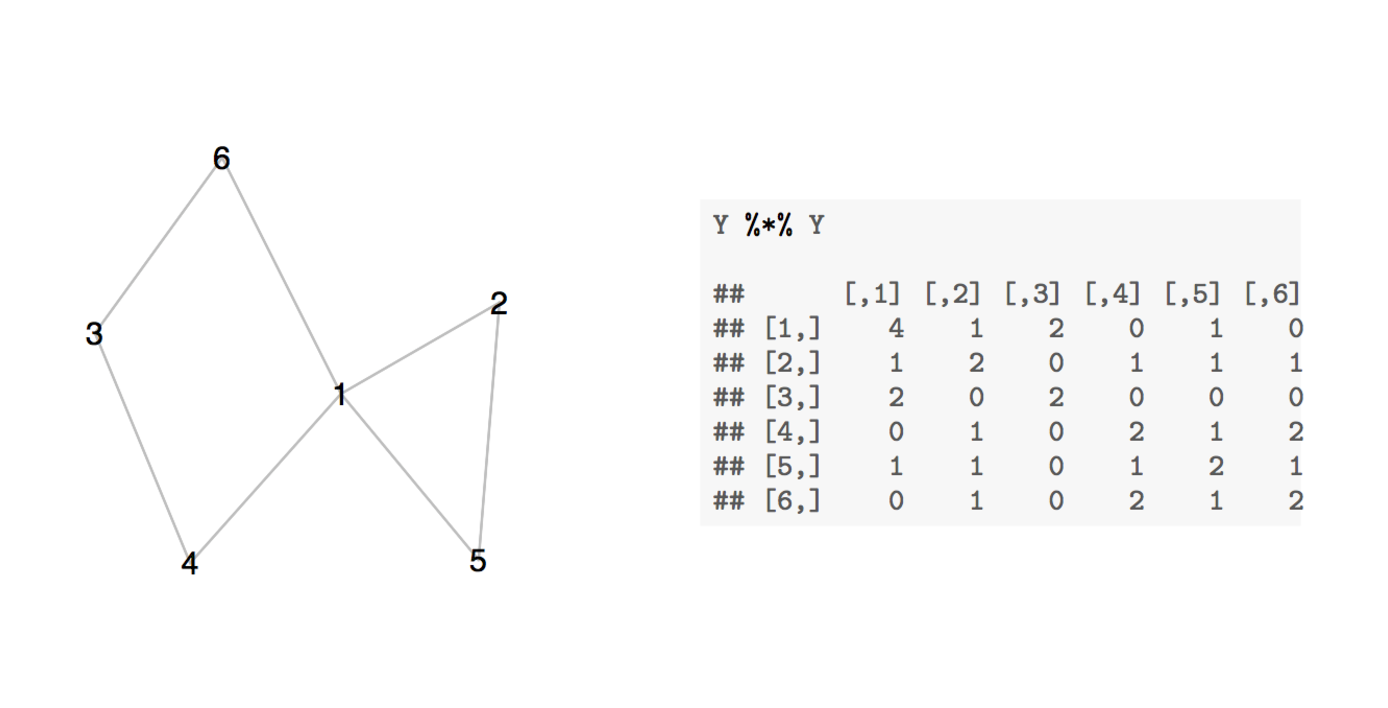
\includegraphics[scale=0.4]{Figs/path}
	\end{figure}
	\vspace{0.1cm}
	
	\begin{itemize}
	\item How many walks of length 2 are there from $i$ to $i$?
	\item How many walks of length 2 are there from $i$ to $j$?
	\end{itemize}
\end{frame}

\begin{frame}{Descriptive SNA III: Path, walk, and distance}
Define $X^{(k)}$, where $k = 1, \cdots, n-1$:
	\begin{equation}
	\begin{split}
	& X^{1} = A \\
	& X^{2} = A + A^{2} \\
	& \vdots \\
	& X^{k} = A + A^{2} + A^{3} + \cdots + A^{k}
	\end{split}
	\end{equation}
Note:
	\begin{itemize}
		\item $X^{(1)}$ counts the number of walks of length 1 between nodes.
		\item $X^{(2)}$ counts the number of walks of length $\leq 2$ between nodes.
		\item $X^{(k)}$ counts the number of walks of length $\leq k$ between nodes.
	\end{itemize}
\end{frame}

\begin{frame}{Descriptive SNA III: Path, walk, and distance}
Altogether, we can define $d_{ij}$, the geodesic distance between $i$ and $j$, as follows. Recall a path is a walk.
	\begin{equation}
	\begin{split}
	d_{ij} & = \text{length of the shortest path between $i$ and $j$} \\
	& = \text{length of the shortest walk between $i$ and $j$} \\
	& = \text{the first or min $k$ for which $A_{ij}^{k}>0$}
	\end{split}
	\end{equation}
\end{frame}

\begin{frame}
Can you write a function in \texttt{R} to compute the geodesic distances for a graph \textbf{A}?
\end{frame}

\begin{frame}

All measures above capture the connectivity of a network.  These connectivity metrics are rather coarse, though.
\end{frame}

\begin{frame}{Descriptive SNA IV: Centrality}

All centrality measures try to capture the \textit{importance} of nodes in a network.
\end{frame}

\begin{frame}{Descriptive SNA IV: Centrality}
\textbf{Degree} centrality uses the degree of a vertex (i.e., the number of neighbors it has) to measure its importance.
	\begin{equation}
	k_i = \sum_j^n A_{ij},
	\end{equation}
where $n$ refers to the number of nodes in the graph.\\

\vspace{0.3cm}
What is the caveat? What does degree centrality not capture?\\

\vspace{0.2cm}
Degree centrality treats all neighbors as ``equal.''
\end{frame}

\begin{frame}{Descriptive SNA IV: Centrality}
\textbf{Eigenvector} centrality measures the influence of a node in a network by giving each vertex a score \textbf{proportional} to the sum of the scores of its neighbors.

	\begin{equation}
	\begin{split}
	& x_i = \frac{1}{\lambda}\sum_j A_{ij}x_j \\
	\Rightarrow \quad & \textbf{Ax} = \lambda\textbf{x},
	\end{split}
	\end{equation}
where $\lambda$ is the leading eigenvector of \textbf{A}.\\

\vspace{0.3cm}
Why do we need eigenvector centrality?
\end{frame}

\begin{frame}{Descriptive SNA IV: Centrality}
\textbf{Closeness} centrality measures the importance of a node by calculating the sum of the length of the shortest paths between the node and all other nodes in the graph.
	\begin{equation}
	c_i = \frac{1}{\frac{1}{n} \sum_j d_{ij}} = \frac{n}{\sum_j d_{ij}},
	\end{equation}
where $d_{ij}$ is the geodesic distance between $i$ and $j$.\\

\vspace{0.3cm}
Use $n$ or $n-1$?  Should we consider the situation such that $i=j$?\\

\vspace{0.2cm}
Maybe not. A vertex's influence on itself is usually not relevant to the working of the network.
\end{frame}

\begin{frame}{Descriptive SNA IV: Centrality}
\textbf{Betweenness} centrality measures the importance of a node by considering how often a node sits on the paths between all other nodes in the graph.
	\begin{equation}
	x_i = \sum \frac{\sigma_{ijk}}{\sigma_{jk}},
	\end{equation}
where $i\neq j\neq k$:
	\begin{itemize}
	\item $\sigma_{jk}$ refers to the number of shortest paths from $j$ to $k$.
	\item $\sigma_{ijk}$ refers to the number of those paths that pass through $i$.
	\end{itemize}

\vspace{0.3cm}
Normalization?\\

\vspace{0.3cm}
One choice is to normalize the path count by dividing by the total number of vertex pairs (i.e., $n^2$).
\end{frame}

\begin{frame}{Descriptive SNA IV: Centrality}
A node in a graph can be important if...

	\begin{itemize}
		\item it connects to many other nodes in the graph.	
		\item it connects to other nodes that connects to many other nodes in the graph.
		\item it is on the paths between many other nodes in the graph.
		\item it is on average close to many other nodes in the graph.
		\item ... and more.
	\end{itemize}

\vspace{0.3cm}
Which one to use?
\end{frame}

\begin{frame}{Descriptive SNA IV: Centrality}
What if we are dealing with a directed network?

	\begin{itemize}
		\item Katz centrality (to avoid zero centrality).
		\item PageRank (designed by Google to avoid inappropriate high centrality).
		\item Hubs and authorities (by taking edge directions seriously; what makes a node more important --- a vertex has high centrality if those that point to it have high centrality OR a vertex high centrality if it points to others with high centrality?).
	\end{itemize}

\vspace{0.3cm}
Your personal website.
\end{frame}

\begin{frame}{Social network analysis (SNA): Two pillars}
	\begin{itemize}
		\item Descriptive: Study numerical summary measures of networks
		\item Generative: Study underlying dynamic process of network formation; hypothesis testing; simulation (e.g., ERGM)
	\end{itemize}
\end{frame}

\begin{frame}{Generative SNA}
	\begin{itemize}
		\item What is a model?  We hope to specify a stochastic model to understand the uncertainty associated with observed outcomes (i.e., networks).
		\item Different (often unobserved) social and interactive processes can lead to similar networks (e.g., assortative mixing and transitivity).
	\end{itemize}
\end{frame}

\begin{frame}{Generative SNA: Bernoulli (Erdos-Renyi) models}
Suppose $Y_{ij}$ in a graph are independent $\forall i,j$:
	\begin{equation}
	\text{logit}[P(Y_{ij}=1 | X=x,\beta)] = \sum_k \beta_k X_{k,ij},
	\end{equation}
given some covariates $X =\{X_1, \cdots, X_k\}$.\\
\vspace{0.2cm}

The log of the likelihood is then
	\begin{equation}
	\ell(\beta|Y,x) \equiv \log[P(Y=y|X=x,\beta)],
	\end{equation}
where $\beta \in \mathbb{R}^{k}$.
\end{frame}

\begin{frame}{Generative SNA: Bernoulli (Erdos-Renyi) models}
$Y_{ij}$ are independent and equally likely
	\begin{equation}
	P(Y_{ij}=1 | X=x,\beta) = \frac{\exp(\beta)}{1+\exp(\beta)} \quad \forall i,j.
	\end{equation}
\vspace{0.2cm}

Equivalently,
	\begin{equation}
	\log\text{odds}(Y_{ij}=1 | X=x,\beta) = \beta \quad \forall i,j.
	\end{equation}
\end{frame}

\begin{frame}{Generative SNA: Bernoulli (Erdos-Renyi) models}
More abstractly, we can rewrite the model as follows.
	\begin{equation}
	P(Y_{ij}=1 | X=x,\beta) = \frac{\exp[\beta g(y)]}{[1+\exp(\beta)]^n}.
	\end{equation}
where $g(y)=\sum_i^n y_{ij}$ and $n$ refers to the number of vertices.\\
\vspace{0.1cm}
The log of the likelihood is then
	\begin{equation}
	\ell(\beta|Y,x) = \beta g(y)-n\log[1+\exp(\beta)].
	\end{equation}
This model can be easily extended when we include more covariates.
\end{frame}

\begin{frame}{Generative SNA: Bernoulli (Erdos-Renyi) models}
Our goal is to find $\hat{\beta}$ that maximizes the log-likelihood function $\ell(\beta|Y,x)$.

	\begin{itemize}
		\item Step 1: Treat each network as a random variable.
		\item Step 2: Propose hypothesis (or hypotheses) that define contingencies among tie variables.
		\item Step 3: Identify the specific form to the model based on your hypothesis (or hypotheses).
		\item Step 4: Simplify parameters for interpretations.
		\item Step 5: Estimate and interpret parameters.
		\item Step 6 (additional): Check goodness-of-fit and robustness.
	\end{itemize}
\end{frame}

\begin{frame}{Practice: French financial elite network (Kadushin 1995, AJS)}
	\begin{itemize}
		\item Each node is a member of french financial elite ($n=28$).
		\item Each edge represents who-to-whom responses to questions about ``who were friends.''
		\item He also recorded a large amount of information on their individual backgrounds and characteristics.
	\end{itemize}
\vspace{0.2cm}
Open \texttt{Practice.R}.
\end{frame}

\begin{frame}[fragile]
\begin{verbatim}
> fit = ergm(ffef ~ edges)
> summary(fit)

==========================
Summary of model fit
==========================

Formula:   ffef ~ edges

Iterations:  5 out of 20 

Monte Carlo MLE Results:
      Estimate Std. Error MCMC % p-value    
edges  -1.5533     0.1355      0  <1e-04 ***
---
Signif. codes:  0 `***' 0.001 `**' 0.01 `*' 0.05 `.' 0.1 ` ' 1

     Null Deviance: 524.0  on 378  degrees of freedom
 Residual Deviance: 350.1  on 377  degrees of freedom
 
AIC: 352.1    BIC: 356    (Smaller is better.) 
\end{verbatim}
\end{frame}

\begin{frame}
How do we interpret the coefficient? Recall
	\begin{equation}
	P(Y_{ij}=1 | X=x,\beta) = \frac{\exp(\beta)}{1+\exp(\beta)} \quad \forall i,j.
	\end{equation}
Therefore,
	\begin{equation}
	P(Y_{ij}=1 | \hat{\beta}) = \frac{\exp(\hat{\beta})}{1+\exp(\hat{\beta})}=0.1746032.
	\end{equation}
What does this number mean?  Degree, density, or..?
\end{frame}

\begin{frame}{Data sources I: Analyze existing network data}
	\begin{itemize}	
	%\item Duke Network Analysis Center: \texttt{https://dnac.ssri.duke.edu/datasets.php}\\
	\item Katya Ognyanova's collection: \texttt{http://kateto.net/2016/05/network-datasets/}\\
	\item Mark Newman's (Univ of Michigan, Ann Arbor) collection: \texttt{http://www-personal.umich.edu/$\sim$mejn/netdata/}
	%\item Stanford Large Network Dataset Collection: \texttt{https://snap.stanford.edu/data/}\\
	\item Koblenz Network Collection: \texttt{http://konect.uni-koblenz.de/}
	\item UCI Network Data Repository: \texttt{https://networkdata.ics.uci.edu/}
	\item ... and more
	\end{itemize}
\end{frame}

\begin{frame}{Data sources II: Collect your own data}

	\begin{itemize}
		\item Surveys and interviews
		\item Archives and other 3rd-party records
		\item Experiment
	\end{itemize}
\end{frame}

\begin{frame}{Examples of SNA research in comparative politics (or political science in general)}

	\begin{itemize}
	\item State-building (e.g., Acemoglu et al 2015 AER)
	\item Regime change (e.g., Linos 2011 AJPS; Naidu et al 2015 WP)
	\item Information diffusion (e.g., Larson and Lewis 2017 APSR)
	\item Voting and electoral accountability (e.g., Arias et al 2017 WP; Cruz et al 2017 AER)
	\item Legislative behaviors and coalition politics (e.g., Bratton and Rouse 2011 LSQ)
	\item Collective action and protests (e.g., Siegel 2011 JOP)
	\item ... and more
	\end{itemize}
\end{frame}

\begin{frame}{Before you start}
	\begin{itemize}
		\item Reflect on your area(s) of substantive interest.
		\item Pick a particular structure/phenomenon/pattern of ``relations.''
			\begin{itemize}
			\item What would the nodes represent?
			\item What would the edges represent?
			\item Should you use an undirected or a directed network?
			\item Should you use a weighted or binary network?
			\item Should you use an unipartite or bipartite?
			\end{itemize}
		\item Describe how it might be represented using networks.
		\item Reflect on the advantages and disadvantages of your chosen representation.
	\end{itemize}
\end{frame}

\begin{frame}
Thank you!\\
\vspace{0.3cm}
\texttt{ccheng11@ucla.edu}
\end{frame}

\begin{frame}{Future directions}
	\begin{itemize}
		\item Causal inferences
		\item Machine learning
	\end{itemize}
\end{frame}

\end{document}
